% *******************************************************************
% STOP - Bitte zuerst lesen, bevor Sie weitermachen
%
% Einige Dinge müssen Sie an Ihre Bedürfnisse (und die Vorgaben Ihres
% Betreuers anpassen).
%
% 1. Sprache
% Das Template unterstützt Deutsch und Englisch, Standard ist Deutsch.
% Wenn Sie Englisch verwenden wollen, ändern Sie bitte direkt am Anfang
% dieser Datei den Eintrag
%    \newcommand{\hsmasprache}{de}
% auf
%    \newcommand{\hsmasprache}{en}
%
% 2. Zitierstil
% Abhängig von dem gewünschten Zitierstil passen Sie bitte in
% preambel.tex die Einstellungen bei \usepackage[backend=biber...
% an. Wie ist dort genau erklärt.
% Achtung: Wenn Sie als Zitierstil Fußnoten wählen bzw. generell
% -------  mit Fußnoten arbeiten, dann beachten Sie bitte, dass
%          Fußnoten in Bildunterschriften und Tabellenüberschriften
%          nicht funktionieren.
%          Siehe hierzu https://texfaq.org/FAQ-ftncapt
%          und https://texfaq.org/FAQ-footintab
%          Sinnvollerweise verzichten Sie auf Fußnoten an diesen
%          Stellen und fügen Quellen einfach per \parancite ein.
%
% 3. Doppelseitiger oder einseitiger Druck
% Das Template ist für doppelseitigen Druck eingestellt. Wollen Sie
% einseitig drucken, müssen Sie in preambel.tex die Einstellungen
% für \documentclass ändern. Und zwar von twoside=on auf twoside=off.
%
% 4. Abkürzungen auf richtige Breite einstellen und sortieren
% In der Datei kapitel/abkuerzungen.tex müssen Sie die _längste_
% Abkürzung in die eckigen Klammern von \begin{acronym} schreiben,
% sonst werden die Abkürzungen nicht richtig ausgerichtet.
% Also z.B. \begin{acronym}[DSGVO].
% Außerdem müssen Sie die Abkürzungen selbst (manuell) sortieren,
% da dies nicht automatisch passiert. Am einfachsten verwenden Sie
% hierzu die Sortierfunktion Ihres Texteditors.
%
% 5. Unnötige Teile entfernen
% Entfernen Sie die Teile, die Sie nicht brauchen, z.B. Anhänge,
% Quelltextverzeichnis etc. Siehe unten
%
% 6. Silbentrennung
% LaTeX führt eine automatische Silbentrennung durch. Allerdings
% werden Wörter, die bereits einen Bindestrich enthalten nicht
% getrennt, z.B. Datenschutz-Grundverordnung. Wenn Sie Ihren Text auf
% Deutsch schreiben, können Sie dann alternativ "= für den Bindestrich
% im Wort verwenden, z.B. Datenschutz"=Grundverordnung, damit LaTeX
% weiterhin richtig trennt.
% Ist die Silbentrennung aus einem anderen Grund nicht erfolgt, sodass
% das Wort über den rechten Rand hinaussteht oder wenn Sie eine weitere
% Trennstelle wollen, können Sie LaTeX helfen, indem Sie weitere
% Trennstellen angeben. Dies geschieht durch "- als Zeichen, z.B.
% Staats"-vertrag.
%
% 7. Nummerierung der Fußnoten
% LaTeX beginnt die Nummerierung der Fußnoten in jedem Kapitel wieder
% bei 1. Manche Dozenten wollen aber eine durchlaufende Nummerierung
% über die gesamte Arbeit. In diesem Fall gehen Sie in die preambel.tex
% und kommentieren den Befehl \counterwithout{footnote}{chapter} ein.
% *******************************************************************

% Sprache für das Dokument festlegen
\newcommand{\hsmasprache}{de} % de oder en für Deutsch oder Englisch

% Preambel mit Einstellungen importieren
% Dokumententyp und benutzte Pakete
\documentclass[open=right,  % Kapitel darf nur auf rechten Seite beginnen
    paper=a4,               % DIN-A4-Papier
    fontsize=12pt,          % Schriftgöße
    headings=small,         % Kleine Überschriften
    headsepline=true,       % Trennlinie am Kopf der Seite
    footsepline=false,      % Keine Trennlinie am Fuß der Seite
    bibliography=totoc,     % Literaturverzeichnis in das Inhaltsverzeichnis aufnehmen
    twoside=on,             % Doppelseitiger Druck - auf off stellen für einseitig
    DIV=7,                  % Verhältnis der Ränder zum bedruckten Bereich
    chapterprefix=true,     % Kapitel x vor dem Kapitelnamen
    cleardoublepage=plain]{scrbook}

% Pakete einbinden, die benötigt werden
\usepackage{ifthen}               % Logische Bedingungen mit ifthenelse
\usepackage{scrlayer-scrpage}
\usepackage[utf8]{inputenc}       % Dateien in UTF-8 benutzen
\usepackage[T1]{fontenc}          % Zeichenkodierung
\usepackage{graphicx}             % Bilder einbinden
\usepackage{enumitem}             % Eigene Listen definieren können

% Setzen von Optionen abhängig von der gewählten Sprache. Die Sprache wird
% in thesis.tex gesetzt.
\ifthenelse{\equal{\hsmasprache}{de}}%
  {%
   \usepackage[main=ngerman, english]{babel}  % Deutsche Sprachunterstützung
   \usepackage[autostyle=true,german=quotes]{csquotes} % Deutsche Anführungszeichen
   \usepackage[pagebackref=false,german]{hyperref} % Hyperlinks
   \newcommand{\hsmasortlocale}{de_DE} % Sortierung der Literatur
  }%
  {%
   \usepackage[main=english, ngerman]{babel} % Englische Sprachunterstützung
   \usepackage[autostyle=true,english=american]{csquotes} % Englische Anführungszeichen
   \usepackage[pagebackref=false,english]{hyperref}  % Hyperlinks
   \newcommand{\hsmasortlocale}{en_US} % Sortierung der Literatur
  }%

\usepackage{xcolor}               % Unterstützung für Farben
\usepackage{amsmath}              % Mathematische Formeln
\usepackage{amsfonts}             % Mathematische Zeichensätze
\usepackage{amssymb}              % Mathematische Symbole
\usepackage{float}                % Fließende Objekte (Tabellen, Grafiken etc.)
\usepackage{booktabs}             % Korrekter Tabellensatz
\usepackage[printonlyused]{acronym}  % Abkürzungsverzeichnis [nur verwendete Abkürzungen]
\usepackage{makeidx}              % Sachregister
\usepackage{listings}             % Quelltexte
\usepackage{listingsutf8}         % Quelltexte in UTF8
\usepackage[hang,font={sf,footnotesize},labelfont={footnotesize,bf}]{caption} % Beschriftungen
\usepackage[scaled]{helvet}       % Schrift Helvetia laden
\usepackage[absolute]{textpos}    % Absolute Textpositionen (für Deckblatt)
\usepackage{calc}                 % Berechnung von Positionen
\usepackage{blindtext}            % Blindtexte
\usepackage[bottom=40mm,left=35mm,right=35mm,top=30mm]{geometry} % Ränder ändern
\usepackage{setspace}             % Abstände korrigieren
\usepackage{scrhack}              % tocbasic Warnung entfernen
\usepackage[all]{hypcap}          % Korrekte Verlinkung von Floats
\usepackage{tabularx}             % Spezielle Tabellen
\usepackage[backend=biber,
  isbn=false,                     % ISBN nicht anzeigen, gleiches geht mit nahezu allen anderen Feldern
  sortlocale=\hsmasortlocale,     % Sortierung der Einträge für Deutsch
                                  %      de_DE: für Deutsch
                                  %      en_US: für Englisch
  autocite=inline,                % regelt Aussehen für \autocite
                                  %      inline: Zitat in Klammern (\parancite)
                                  %      footnote: Zitat in Fußnoten (\footcite)
                                  %      plain: Zitat direkt ohne Klammern (\cite)
  style=authoryear,               % Legt den Stil für die Zitate fest
                                  %      ieee: Zitate als Zahlen [1]
                                  %      alphabetic: Zitate als Kürzel und Jahr [Ein05]
                                  %      authoryear: Zitate Author und Jahr [Einstein (1905)]
  hyperref=true,                  % Hyperlinks für Zitate
  firstinits=false                % Vornamen abkürzen (Maier, M. anstatt Maier, Markus)?
                                  %      true: abkürzen
                                  %      false: nicht abkürzen
]{biblatex}                       % Literaturverwaltung mit BibLaTeX
\usepackage{rotating}             % Seiten drehen
\usepackage{harveyballs}          % Harveyballs
\usepackage{chngcntr}             % Counter (Zähler) ändern können - für Fußnotennummern

% Einstellungen zu den Fußnoten
\renewcommand{\footnotesize}{\fontsize{9}{10}\selectfont} % Größe der Fußnoten
\setlength{\footnotesep}{8pt} % Abstand zwischen den Fußnoten

% Kommentieren Sie diese Zeile ein, wenn Sie eine "durchlaufende" Nummerierung bei den
% Fußnoten wünschen, d.h. wenn die Fußnoten nicht bei jedem Kapitel wieder bei 1
% beginnen sollen.
%\counterwithout{footnote}{chapter}

\setlength{\bibitemsep}{1em}      % Abstand zwischen den Literaturangaben
\setlength{\bibhang}{2em}         % Einzug nach jeweils erster Zeile

% Trennung von URLs im Literaturverzeichnis (große Werte [> 10000] verhindern die Trennung)
\defcounter{biburlnumpenalty}{10} % Strafe für Trennung in URL nach Zahl
\defcounter{biburlucpenalty}{500} % Strafe für Trennung in URL nach Großbuchstaben
\defcounter{biburllcpenalty}{500} % Strafe für Trennung in URL nach Kleinbuchstaben

% Farben definieren
\definecolor{linkblue}{RGB}{0, 0, 100}
\definecolor{linkblack}{RGB}{0, 0, 0}
\definecolor{comment}{RGB}{63, 127, 95}
\definecolor{darkgreen}{RGB}{14, 144, 102}
\definecolor{darkblue}{RGB}{0,0,168}
\definecolor{darkred}{RGB}{128,0,0}
\definecolor{javadoccomment}{RGB}{0,0,240}

% Einstellungen für das Hyperlink-Paket
\hypersetup{
    colorlinks=true,      % Farbige links verwenden
%    allcolors=linkblue,
    linktoc=all,          % Links im Inhaltsverzeichnis
    linkcolor=linkblack,  % Querverweise
    citecolor=linkblack,  % Literaturangaben
    filecolor=linkblack,  % Dateilinks
    urlcolor=linkblack    % URLs
}

% Einstellungen für Quelltexte
\lstset{
      xleftmargin=0.2cm,
      basicstyle=\footnotesize\ttfamily,
      keywordstyle=\color{darkgreen},
      identifierstyle=\color{darkblue},
      commentstyle=\color{comment},
      stringstyle=\color{darkred},
      tabsize=2,
      lineskip={2pt},
      columns=flexible,
      inputencoding=utf8,
      captionpos=b,
      breakautoindent=true,
      breakindent=2em,
      breaklines=true,
      prebreak=,
      postbreak=,
      numbers=none,
      numberstyle=\tiny,
      showspaces=false,      % Keine Leerzeichensymbole
      showtabs=false,        % Keine Tabsymbole
      showstringspaces=false,% Leerzeichen in Strings
      morecomment=[s][\color{javadoccomment}]{/**}{*/},
      literate={Ö}{{\"O}}1 {Ä}{{\"A}}1 {Ü}{{\"U}}1 {ß}{{\ss}}2 {ü}{{\"u}}1 {ä}{{\"a}}1 {ö}{{\"o}}1
}

\urlstyle{same}

% Einstellungen für Überschriften
\renewcommand*{\chapterformat}{%
  \Large\chapapp~\thechapter   % Große Schrift
  \vspace{0.3cm}               % Abstand zum Titel des Kapitels
}

% Abstände für die Überschriften setzen
\renewcommand{\chapterheadstartvskip}{\vspace*{2.6cm}}
\renewcommand{\chapterheadendvskip}{\vspace*{1.5cm}}

% Vertikale Abstände für die Überschriften etwas verkleinern
\RedeclareSectionCommand[
  beforeskip=-1.8\baselineskip,
  afterskip=0.25\baselineskip]{section}

\RedeclareSectionCommand[
  beforeskip=-1.8\baselineskip,
  afterskip=0.15\baselineskip]{subsection}

\RedeclareSectionCommand[
  beforeskip=-1.8\baselineskip,
  afterskip=0.15\baselineskip]{subsubsection}

% In der Kopfzeile nur die kurze Kapitelbezeichnung (ohne Kapitel davor)
\renewcommand*\chaptermarkformat{\thechapter\autodot\enskip}
\automark[chapter]{chapter}

% Einstellungen für Schriftarten
\setkomafont{pagehead}{\normalfont\sffamily}
\setkomafont{pagenumber}{\normalfont\sffamily}
\setkomafont{paragraph}{\sffamily\bfseries\small}
\setkomafont{subsubsection}{\sffamily\itshape\bfseries\small}
\addtokomafont{footnote}{\footnotesize}
\setkomafont{chapter}{\LARGE\selectfont\bfseries}

% Wichtige Abstände
\setlength{\parskip}{0.2cm}  % 2mm Abstand zwischen zwei Absätzen
\setlength{\parindent}{0mm}  % Absätze nicht einziehen
\clubpenalty = 10000         % Keine "Schusterjungen"
\widowpenalty = 10000        % Keine "Hurenkinder"
\displaywidowpenalty = 10000 % Keine "Hurenkinder"
                             % Siehe: https://de.wikipedia.org/wiki/Hurenkind_und_Schusterjunge

% Index erzeugen
\makeindex

% Einfacher Font-Wechsel über dieses Makro
\newcommand{\changefont}[3]{
\fontfamily{#1} \fontseries{#2} \fontshape{#3} \selectfont}

% Eigenes Makro für Bilder. Das label (für \ref) ist dann einfach
% der Name der Bilddatei
\newcommand{\bild}[3]{
\begin{figure}[ht]
  \centering
  \includegraphics[width=#2]{#1}
  \caption{#3}
  \label{#1}
\end{figure}}

% Wo liegt Sourcecode?
\newcommand{\srcloc}{src/}

% Wo sind die Bilder?
\graphicspath{{bilder/}}

% Makros für typographisch korrekte Abkürzungen
\newcommand{\zb}[0]{z.\,B.}
\newcommand{\dahe}[0]{d.\,h.}
\newcommand{\ua}[0]{u.\,a.}

% Flags für Veröffentlichung und Sperrvermerk
\newboolean{hsmapublizieren}
\newboolean{hsmasperrvermerk}

% Tabellenzellen mit mehreren Zeilen
\newcolumntype{L}{>{\raggedright\arraybackslash}X}
\newcolumntype{b}{l}
\newcolumntype{s}{>{\hsize=.3\hsize}l}
\newcolumntype{F}{>{\hsize=\dimexpr2\hsize+2\tabcolsep+\arrayrulewidth\relax}X}

% Checklisten mit zwei Ebenen
\newlist{checklist}{itemize}{2}
\setlist[checklist]{label=$\square$}

% Dokumenteninfos importieren
% -------------------------------------------------------
% Daten für die Arbeit
% Wenn hier alles korrekt eingetragen wurde, wird das Titelblatt
% automatisch generiert. D.h. die Datei titelblatt.tex muss nicht mehr
% angepasst werden.

% Titel der Arbeit auf Deutsch
\newcommand{\hsmatitelde}{Einsatz eines Flux-Kompensators für Zeitreisen mit einer maximalen Höchstgeschwindigkeit von WARP~7}

% Titel der Arbeit auf Englisch
\newcommand{\hsmatitelen}{Application of a flux compensator for timetravel with a maximum velocity of warp~7}

% Weitere Informationen zur Arbeit
\newcommand{\hsmaort}{Mannheim}    % Ort
\newcommand{\hsmaautorvname}{Max} % Vorname(n)
\newcommand{\hsmaautornname}{Mustermann} % Nachname(n)
\newcommand{\hsmadatum}{24.10.2019} % Datum der Abgabe
\newcommand{\hsmajahr}{2019} % Jahr der Abgabe
\newcommand{\hsmafirma}{Paukenschlag GmbH, Mannheim} % Firma bei der die Arbeit durchgeführt wurde
\newcommand{\hsmabetreuer}{Prof. Peter Mustermann, Hochschule Mannheim} % Betreuer an der Hochschule
\newcommand{\hsmazweitkorrektor}{Erika Mustermann, Paukenschlag GmbH} % Betreuer im Unternehmen oder Zweitkorrektor
\newcommand{\hsmafakultaet}{I} % I für Informatik oder E, S, B, D, M, N, W, V
\newcommand{\hsmastudiengang}{IB} % IB IMB UIB CSB IM MTB (weitere siehe titleblatt.tex)

% Zustimmung zur Veröffentlichung
\setboolean{hsmapublizieren}{true}   % Einer Veröffentlichung wird zugestimmt
\setboolean{hsmasperrvermerk}{false} % Die Arbeit hat keinen Sperrvermerk

% -------------------------------------------------------
% Abstract
% Achtung: Wenn Sie im Abstrakt Anführungszeichen verwenden wollen, dann benutzen Sie
%          nicht "` und "', sondern \enquote{}. "` und "' werden nicht richtig
%          erkannt.

% Kurze (maximal halbseitige) Beschreibung, worum es in der Arbeit geht auf Deutsch
\newcommand{\hsmaabstractde}{Jemand musste Josef K. verleumdet haben, denn ohne dass er etwas Böses getan hätte, wurde er eines Morgens verhaftet. Wie ein Hund! sagte er, es war, als sollte die Scham ihn überleben. Als Gregor Samsa eines Morgens aus unruhigen Träumen erwachte, fand er sich in seinem Bett zu einem ungeheueren Ungeziefer verwandelt. Und es war ihnen wie eine Bestätigung ihrer neuen Träume und guten Absichten, als am Ziele ihrer Fahrt die Tochter als erste sich erhob und ihren jungen Körper dehnte. Es ist ein eigentümlicher Apparat, sagte der Offizier zu dem Forschungsreisenden und überblickte mit einem gewissermaßen bewundernden Blick den ihm doch wohl bekannten Apparat. Sie hätten noch ins Boot springen können, aber der Reisende hob ein schweres, geknotetes Tau vom Boden, drohte ihnen damit und hielt sie dadurch von dem Sprunge ab. In den letzten Jahrzehnten ist das Interesse an Künstlern sehr zurückgegangen. Aber sie überwanden sich, umdrängten den Käfig und wollten sich gar nicht fortrühren.}

% Kurze (maximal halbseitige) Beschreibung, worum es in der Arbeit geht auf Englisch
\newcommand{\hsmaabstracten}{The European languages are members of the same family. Their separate existence is a myth. For science, music, sport, etc, Europe uses the same vocabulary. The languages only differ in their grammar, their pronunciation and their most common words. Everyone realizes why a new common language would be desirable: one could refuse to pay expensive translators. To achieve this, it would be necessary to have uniform grammar, pronunciation and more common words. If several languages coalesce, the grammar of the resulting language is more simple and regular than that of the individual languages. The new common language will be more simple and regular than the existing European languages. It will be as simple as Occidental; in fact, it will be Occidental. To an English person, it will seem like simplified English, as a skeptical Cambridge friend of mine told me what Occidental is.}


% Literatur-Datenbank
% \addbibresource{literatur.bib}   % BibLaTeX-Datei mit Literaturquellen einbinden
\addbibresource{library.bib}   % BibLaTeX-Datei mit Literaturquellen einbinden

% Anfang des Dokuments
\begin{document}
\frontmatter

% Römische Ziffern für die "Front-Matter"
\setcounter{page}{0}
\changefont{ptm}{m}{n}  % Times New Roman für den Fließtext
\renewcommand{\rmdefault}{ptm}

% Titelblatt
% *******************************************************************
% In dieser Datei sollten eigentlich keine Veränderungen
% notwendig sein. Alle Einstellungen erfolgen in docinfo.tex und
% der thesis.tex.
% *******************************************************************

\thispagestyle{empty}

% Fakultäten der HS-Mannheim
% *******************************************************************
\ifthenelse{\equal{\hsmafakultaet}{I}}%
  {\newcommand{\hsmafakultaetlangde}{Fakultät für Informatik}%
   \newcommand{\hsmafakultaetlangen}{Department of Computer Science}}{}

\ifthenelse{\equal{\hsmafakultaet}{E}}%
  {\newcommand{\hsmafakultaetlangde}{Fakultät für Elektrotechnik}%
   \newcommand{\hsmafakultaetlangen}{Department of Electrical Engineering}}{}

\ifthenelse{\equal{\hsmafakultaet}{S}}%
  {\newcommand{\hsmafakultaetlangde}{Fakultät für Sozialwesen}%
   \newcommand{\hsmafakultaetlangen}{Department of Social Work}}{}

\ifthenelse{\equal{\hsmafakultaet}{B}}%
  {\newcommand{\hsmafakultaetlangde}{Fakultät für Biotechnologie}%
   \newcommand{\hsmafakultaetlangen}{Department of Biotechnology}}{}

\ifthenelse{\equal{\hsmafakultaet}{D}}%
  {\newcommand{\hsmafakultaetlangde}{Fakultät für Gestaltung}%
   \newcommand{\hsmafakultaetlangen}{Department of Design}}{}

\ifthenelse{\equal{\hsmafakultaet}{M}}%
  {\newcommand{\hsmafakultaetlangde}{Fakultät für Maschinenbau}%
   \newcommand{\hsmafakultaetlangen}{Department of Mechanical Engineering}}{}

\ifthenelse{\equal{\hsmafakultaet}{N}}%
  {\newcommand{\hsmafakultaetlangde}{Fakultät für Informationstechnik}%
   \newcommand{\hsmafakultaetlangen}{Department of Information Technology}}{}

\ifthenelse{\equal{\hsmafakultaet}{W}}%
  {\newcommand{\hsmafakultaetlangde}{Fakultät für Wirtschaftsingenieurwesen}%
   \newcommand{\hsmafakultaetlangen}{Department of Engineering and Management}}{}

\ifthenelse{\equal{\hsmafakultaet}{V}}%
  {\newcommand{\hsmafakultaetlangde}{Fakultät für Verfahrens- und Chemietechnik}%
   \newcommand{\hsmafakultaetlangen}{Department of Chemical Process Engineering}}{}

% Studiengänge der HS-Mannheim
% *******************************************************************
\ifthenelse{\equal{\hsmastudiengang}{IB}}%
  {\newcommand{\hsmastudienganglangde}{Informatik}%
  \newcommand{\hsmastudienganglangen}{Computer Science}%
  \newcommand{\hsmatypde}{Bachelor-Thesis}%
  \newcommand{\hsmatypen}{Bachelor Thesis}%
  \newcommand{\hsmagrad}{\hsmabsc}}{}

\ifthenelse{\equal{\hsmastudiengang}{IMB}}%
  {\newcommand{\hsmastudienganglangde}{Medizinische Informatik}%
  \newcommand{\hsmastudienganglangen}{Medical Informatics}%
  \newcommand{\hsmatypde}{Bachelor-Thesis}%
  \newcommand{\hsmatypen}{Bachelor Thesis}%
  \newcommand{\hsmagrad}{\hsmabsc}}{}

\ifthenelse{\equal{\hsmastudiengang}{UIB}}%
  {\newcommand{\hsmastudienganglangde}{Unternehmens- und Wirtschaftsinformatik}%
  \newcommand{\hsmastudienganglangen}{Enterprise Computing}%
  \newcommand{\hsmatypde}{Bachelor-Thesis}%
  \newcommand{\hsmatypen}{Bachelor Thesis}%
  \newcommand{\hsmagrad}{\hsmabsc}}{}

\ifthenelse{\equal{\hsmastudiengang}{CSB}}%
  {\newcommand{\hsmastudienganglangde}{Cyber Security}%
  \newcommand{\hsmastudienganglangen}{Cyber Security}%
  \newcommand{\hsmatypde}{Bachelor-Thesis}%
  \newcommand{\hsmatypen}{Bachelor Thesis}%
  \newcommand{\hsmagrad}{\hsmabsc}}{}

\ifthenelse{\equal{\hsmastudiengang}{IM}}%
  {\newcommand{\hsmastudienganglangde}{Informatik}%
   \newcommand{\hsmastudienganglangen}{Computer Science}%
   \newcommand{\hsmatypde}{Master-Thesis}%
   \newcommand{\hsmatypen}{Master Thesis}%
   \newcommand{\hsmagrad}{\hsmamaster}}{}

\ifthenelse{\equal{\hsmastudiengang}{MEB}}%
  {\newcommand{\hsmastudienganglangde}{Mechatronik}%
   \newcommand{\hsmastudienganglangen}{Mechatronic}%
   \newcommand{\hsmatypde}{Bachelor-Thesis}%
   \newcommand{\hsmatypen}{Bachelor Thesis}%
   \newcommand{\hsmagrad}{\hsmabsc}}{}

\ifthenelse{\equal{\hsmastudiengang}{UB}}%
  {\newcommand{\hsmastudienganglangde}{Automatisierungstechnik}%
   \newcommand{\hsmastudienganglangen}{Automation Technology}%
   \newcommand{\hsmatypde}{Bachelor-Thesis}%
   \newcommand{\hsmatypen}{Bachelor Thesis}%
   \newcommand{\hsmagrad}{\hsmabsc}}{}

\ifthenelse{\equal{\hsmastudiengang}{ELB}}%
  {\newcommand{\hsmastudienganglangde}{Elektro- und Informationstechnik/Ingenieurpädagogik}%
   \newcommand{\hsmastudienganglangen}{Elektro- und Informationstechnik/Ingenieurpädagogik}%
   \newcommand{\hsmatypde}{Bachelor-Thesis}%
   \newcommand{\hsmatypen}{Bachelor Thesis}%
   \newcommand{\hsmagrad}{\hsmabsc}}{}

\ifthenelse{\equal{\hsmastudiengang}{EBE}}%
  {\newcommand{\hsmastudienganglangde}{Energietechnik und erneuerbare Energien}%
   \newcommand{\hsmastudienganglangen}{Power Engineering ans Renewable Energies}%
   \newcommand{\hsmatypde}{Bachelor-Thesis}%
   \newcommand{\hsmatypen}{Bachelor Thesis}%
   \newcommand{\hsmagrad}{\hsmabsc}}{}

\ifthenelse{\equal{\hsmastudiengang}{TS}}%
  {\newcommand{\hsmastudienganglangde}{Translation Studies}%
   \newcommand{\hsmastudienganglangen}{Translation Studies}%
   \newcommand{\hsmatypde}{Bachelor-Thesis}%
   \newcommand{\hsmatypen}{Bachelor Thesis}%
   \newcommand{\hsmagrad}{\hsmabsc}}{}

\ifthenelse{\equal{\hsmastudiengang}{EM}}%
  {\newcommand{\hsmastudienganglangde}{Automatisierungs- und Energiesysteme}%
   \newcommand{\hsmastudienganglangen}{Automation and Energy Systems}%
   \newcommand{\hsmatypde}{Master-Thesis}%
   \newcommand{\hsmatypen}{Master Thesis}%
   \newcommand{\hsmagrad}{\hsmamaster}}{}

\ifthenelse{\equal{\hsmastudiengang}{ELM}}%
  {\newcommand{\hsmastudienganglangde}{Lehramt Ingenieurpädagogik}%
   \newcommand{\hsmastudienganglangen}{Lectureship Educational Engineering}%
   \newcommand{\hsmatypde}{Master-Thesis}%
   \newcommand{\hsmatypen}{Master Thesis}%
   \newcommand{\hsmagrad}{\hsmamaster}}{}

\ifthenelse{\equal{\hsmastudiengang}{SAB}}%
  {\newcommand{\hsmastudienganglangde}{Soziale Arbeit}%
   \newcommand{\hsmastudienganglangen}{Social Labour}%
   \newcommand{\hsmatypde}{Bachelor-Thesis}%
   \newcommand{\hsmatypen}{Bachelor Thesis}%
   \newcommand{\hsmagrad}{\hsmaba}}{}

\ifthenelse{\equal{\hsmastudiengang}{SAM}}%
  {\newcommand{\hsmastudienganglangde}{Soziale Arbeit}%
   \newcommand{\hsmastudienganglangen}{Social Labour}%
   \newcommand{\hsmatypde}{Master-Thesis}%
   \newcommand{\hsmatypen}{Master Thesis}%
   \newcommand{\hsmagrad}{\hsmamastera}}{}

\ifthenelse{\equal{\hsmastudiengang}{BB}}%
  {\newcommand{\hsmastudienganglangde}{Biotechnology}%
   \newcommand{\hsmastudienganglangen}{Biotechnology}%
   \newcommand{\hsmatypde}{Bachelor-Thesis}%
   \newcommand{\hsmatypen}{Bachelor Thesis}%
   \newcommand{\hsmagrad}{\hsmabsc}}{}

\ifthenelse{\equal{\hsmastudiengang}{BCB}}%
  {\newcommand{\hsmastudienganglangde}{Biologische Chemie}%
   \newcommand{\hsmastudienganglangen}{Biological Chemics}%
   \newcommand{\hsmatypde}{Bachelor-Thesis}%
   \newcommand{\hsmatypen}{Bachelor Thesis}%
   \newcommand{\hsmagrad}{\hsmabsc}}{}

\ifthenelse{\equal{\hsmastudiengang}{BMEBST}}%
  {\newcommand{\hsmastudienganglangde}{Biotechnology - Biomedical Science and Technology}%
   \newcommand{\hsmastudienganglangen}{Biotechnology - Biomedical Science and Technology}%
   \newcommand{\hsmatypde}{Master-Thesis}%
   \newcommand{\hsmatypen}{Master Thesis}%
   \newcommand{\hsmagrad}{\hsmamaster}}{}

\ifthenelse{\equal{\hsmastudiengang}{BMEBPD}}%
  {\newcommand{\hsmastudienganglangde}{Biotechnology - Bioprocess Development}%
   \newcommand{\hsmastudienganglangen}{Biotechnology - Bioprocess Development}%
   \newcommand{\hsmatypde}{Master-Thesis}%
   \newcommand{\hsmatypen}{Master Thesis}%
   \newcommand{\hsmagrad}{\hsmamaster}}{}

\ifthenelse{\equal{\hsmastudiengang}{BLSM}}%
  {\newcommand{\hsmastudienganglangde}{Life Science Management}%
   \newcommand{\hsmastudienganglangen}{Life Science Management}%
   \newcommand{\hsmatypde}{Master-Thesis}%
   \newcommand{\hsmatypen}{Master Thesis}%
   \newcommand{\hsmagrad}{\hsmamaster}}{}

\ifthenelse{\equal{\hsmastudiengang}{KDB}}%
  {\newcommand{\hsmastudienganglangde}{Kommunikationsdesign}%
   \newcommand{\hsmastudienganglangen}{Communication Design}%
   \newcommand{\hsmatypde}{Bachelor-Thesis}%
   \newcommand{\hsmatypen}{Bachelor Thesis}%
   \newcommand{\hsmagrad}{\hsmaba}}{}

\ifthenelse{\equal{\hsmastudiengang}{KDM}}%
  {\newcommand{\hsmastudienganglangde}{Kommunikationsdesign}%
   \newcommand{\hsmastudienganglangen}{Communication Design}%
   \newcommand{\hsmatypde}{Master-Thesis}%
   \newcommand{\hsmatypen}{Master Thesis}%
   \newcommand{\hsmagrad}{\hsmamastera}}{}

\ifthenelse{\equal{\hsmastudiengang}{MB}}%
  {\newcommand{\hsmastudienganglangde}{Maschinenbau}%
   \newcommand{\hsmastudienganglangen}{Mechanical Engineering}%
   \newcommand{\hsmatypde}{Bachelor-Thesis}%
   \newcommand{\hsmatypen}{Bachelor Thesis}%
   \newcommand{\hsmagrad}{\hsmabsc}}{}

\ifthenelse{\equal{\hsmastudiengang}{MM}}%
  {\newcommand{\hsmastudienganglangde}{Maschinenbau}%
   \newcommand{\hsmastudienganglangen}{Mechanical Engineering}%
   \newcommand{\hsmatypde}{Master-Thesis}%
   \newcommand{\hsmatypen}{Master Thesis}%
   \newcommand{\hsmagrad}{\hsmamaster}}{}

\ifthenelse{\equal{\hsmastudiengang}{NEB}}%
  {\newcommand{\hsmastudienganglangde}{Elektronik}%
   \newcommand{\hsmastudienganglangen}{Electronics}%
   \newcommand{\hsmatypde}{Bachelor-Thesis}%
   \newcommand{\hsmatypen}{Bachelor Thesis}%
   \newcommand{\hsmagrad}{\hsmabsc}}{}

\ifthenelse{\equal{\hsmastudiengang}{TIB}}%
  {\newcommand{\hsmastudienganglangde}{Technische Informatik}%
   \newcommand{\hsmastudienganglangen}{Technical Information Technology}%
   \newcommand{\hsmatypde}{Bachelor-Thesis}%
   \newcommand{\hsmatypen}{Bachelor Thesis}%
   \newcommand{\hsmagrad}{\hsmabsc}}{}

\ifthenelse{\equal{\hsmastudiengang}{MTB}}%
  {\newcommand{\hsmastudienganglangde}{Medizintechnik}%
   \newcommand{\hsmastudienganglangen}{Medical Technology}%
   \newcommand{\hsmatypde}{Bachelor-Thesis}%
   \newcommand{\hsmatypen}{Bachelor Thesis}%
   \newcommand{\hsmagrad}{\hsmabsc}}{}

\ifthenelse{\equal{\hsmastudiengang}{MTM}}%
  {\newcommand{\hsmastudienganglangde}{Medizintechnik}%
   \newcommand{\hsmastudienganglangen}{Medical Technology}%
   \newcommand{\hsmatypde}{Master-Thesis}%
   \newcommand{\hsmatypen}{Master Thesis}%
   \newcommand{\hsmagrad}{\hsmamaster}}{}

\ifthenelse{\equal{\hsmastudiengang}{NM}}%
  {\newcommand{\hsmastudienganglangde}{Informationstechnik}%
   \newcommand{\hsmastudienganglangen}{Informationstechnik}%
   \newcommand{\hsmatypde}{Master-Thesis}%
   \newcommand{\hsmatypen}{Master Thesis}%
   \newcommand{\hsmagrad}{\hsmamaster}}{}

\ifthenelse{\equal{\hsmastudiengang}{WB}}%
  {\newcommand{\hsmastudienganglangde}{Wirtschaftsingenieurwesen}%
   \newcommand{\hsmastudienganglangen}{Engineering Management}%
   \newcommand{\hsmatypde}{Bachelor-Thesis}%
   \newcommand{\hsmatypen}{Bachelor Thesis}%
   \newcommand{\hsmagrad}{\hsmabsc}}{}

\ifthenelse{\equal{\hsmastudiengang}{WM}}%
  {\newcommand{\hsmastudienganglangde}{Wirtschaftsingenieurwesen}%
   \newcommand{\hsmastudienganglangen}{Engineering Management}%
   \newcommand{\hsmatypde}{Master-Thesis}%
   \newcommand{\hsmatypen}{Master Thesis}%
   \newcommand{\hsmagrad}{\hsmamaster}}{}

\ifthenelse{\equal{\hsmastudiengang}{WMI}}%
  {\newcommand{\hsmastudienganglangde}{Wirtschaftsingenieurwesen}%
   \newcommand{\hsmastudienganglangen}{Engineering Management}%
   \newcommand{\hsmatypde}{Master-Thesis}%
   \newcommand{\hsmatypen}{Master Thesis}%
   \newcommand{\hsmagrad}{\hsmamaster}}{}

\ifthenelse{\equal{\hsmastudiengang}{WMB}}%
  {\newcommand{\hsmastudienganglangde}{Wirtschaftsingenieurwesen mit den\\ ingenieurwissenschaftlichen Fachrichtungen Maschinenbau und Elektrotechnik}%
   \newcommand{\hsmastudienganglangen}{Engineering Management\\ with focus on Mechanical and Electrical Engineering}%
   \newcommand{\hsmatypde}{Master-Thesis}%
   \newcommand{\hsmatypen}{Master Thesis}%
   \newcommand{\hsmagrad}{\hsmamaster}}{}

\ifthenelse{\equal{\hsmastudiengang}{WMW}}%
  {\newcommand{\hsmastudienganglangde}{Wirtschaftsingenieurwesen mit\\ ingenieurwissenschaftlicher Vertiefung des Maschinenbaus}%
   \newcommand{\hsmastudienganglangen}{Engineering Management\\ deepening the engineering aspects of Mechanical Engineering}%
   \newcommand{\hsmatypde}{Master-Thesis}%
   \newcommand{\hsmatypen}{Master Thesis}%
   \newcommand{\hsmagrad}{\hsmamaster}}{}

\ifthenelse{\equal{\hsmastudiengang}{VB}}%
  {\newcommand{\hsmastudienganglangde}{Verfahrenstechnik}%
   \newcommand{\hsmastudienganglangen}{Process Engineering}%
   \newcommand{\hsmatypde}{Bachelor-Thesis}%
   \newcommand{\hsmatypen}{Bachelor Thesis}%
   \newcommand{\hsmagrad}{\hsmabsc}}{}

\ifthenelse{\equal{\hsmastudiengang}{CB}}%
  {\newcommand{\hsmastudienganglangde}{Chemische Technik}%
   \newcommand{\hsmastudienganglangen}{Chemical Engineering}%
   \newcommand{\hsmatypde}{Bachelor-Thesis}%
   \newcommand{\hsmatypen}{Bachelor Thesis}%
   \newcommand{\hsmagrad}{\hsmabsc}}{}

\ifthenelse{\equal{\hsmastudiengang}{CM}}%
  {\newcommand{\hsmastudienganglangde}{Chemieingenieurwesen}%
   \newcommand{\hsmastudienganglangen}{Chemical Engineering}%
   \newcommand{\hsmatypde}{Master-Thesis}%
   \newcommand{\hsmatypen}{Master Thesis}%
   \newcommand{\hsmagrad}{\hsmamaster}}{}

% Abschlüsse
% *******************************************************************
\newcommand{\hsmabsc}{Bachelor of Science (B.Sc.)}
\newcommand{\hsmaba}{Bachelor of Arts (B.A.)}
\newcommand{\hsmamaster}{Master of Science (M.Sc.)}
\newcommand{\hsmamastera}{Master of Arts (M.A.)}
\newcommand{\hsmamasterba}{Master of Business Administration (MBA)}

\newcommand{\hsmakoerperschaftde}{Hochschule Mannheim}
\newcommand{\hsmakoerperschaften}{University of Applied Sciences Mannheim}

\newcommand{\hsmaautorbib}{\hsmaautornname, \hsmaautorvname} % Autor Nachname, Vorname
\newcommand{\hsmaautor}{\hsmaautorvname \ \hsmaautornname} % Autor Vorname Nachname

\ifthenelse{\equal{\hsmasprache}{de}}%
  {\newcommand{\hsmatyp}{\hsmatypde}%
   \newcommand{\hsmathesistype}{zur Erlangung des akademischen Grades \hsmagrad}%
   \newcommand{\hsmakoerperschaft}{\hsmakoerperschaftde}%
   \newcommand{\hsmastudiengangname}{Studiengang \hsmastudienganglangde}%
   \newcommand{\hsmastudienganglang}{\hsmastudienganglangde}%
   \newcommand{\hsmatitel}{\hsmatitelde}%
   \newcommand{\hsmatutor}{Betreuer}%
   \newcommand{\hsmafakultaetlang}{\hsmafakultaetlangde}%
   \newcommand{\hsmalistoftables}{Tabellenverzeichnis}%
   \newcommand{\hsmalistoffigures}{Abbildungsverzeichnis}%
   \newcommand{\hsmalistings}{Quellcodeverzeichnis}%
   \newcommand{\hsmaindex}{Index}%
   \newcommand{\hsmaabbreviations}{Abkürzungsverzeichnis}%
   \newcommand{\hsmasnowcardanforderung}{Anforderung}%
   \newcommand{\hsmasnowcardno}{Nr}%
   \newcommand{\hsmasnowcardart}{Art}%
   \newcommand{\hsmasnowcardprio}{Prio}%
   \newcommand{\hsmasnowcardtitel}{Titel}%
   \newcommand{\hsmasnowcardherkunft}{Herkunft}%
   \newcommand{\hsmasnowcardkonflikt}{Konflikte}%
   \newcommand{\hsmasnowcardbeschreibung}{Beschreibung}%
   \newcommand{\hsmasnowcardfitkriterium}{Fit-Kriterium}%
   \newcommand{\hsmasnowcardmaterial}{Weiteres Material}%
   \newcommand{\hsmaqasanforderung}{QAS}%
   \newcommand{\hsmaqasno}{Nr}%
   \newcommand{\hsmaqasart}{Art}%
   \newcommand{\hsmaqasprio}{Prio}%
   \newcommand{\hsmaqastitel}{Titel}%
   \newcommand{\hsmaqasquelle}{Quelle}%
   \newcommand{\hsmaqasstimulus}{Stimulus}%
   \newcommand{\hsmaqasartefakt}{Artefakt}%
   \newcommand{\hsmaqasumgebung}{Umgebung}%
   \newcommand{\hsmaqasantwort}{Antwort}%
   \newcommand{\hsmaqasmass}{Maß für Antwort}%
   \selectlanguage{ngerman}}%
  {\newcommand{\hsmatyp}{\hsmatypen}%
   \newcommand{\hsmathesistype}{for the acquisition of the academic degree \hsmagrad}%
   \newcommand{\hsmakoerperschaft}{\hsmakoerperschaften}%
   \newcommand{\hsmastudiengangname}{Course of Studies: \hsmastudienganglang}%
   \newcommand{\hsmastudienganglang}{\hsmastudienganglangen}%
   \newcommand{\hsmatitel}{\hsmatitelen}%
   \newcommand{\hsmatutor}{Tutors}
   \newcommand{\hsmafakultaetlang}{\hsmafakultaetlangen}%
   \newcommand{\hsmalistoftables}{List of Tables}%
   \newcommand{\hsmalistoffigures}{List of Figures}%
   \newcommand{\hsmalistings}{Listings}%
   \newcommand{\hsmaindex}{Index}%
   \newcommand{\hsmaabbreviations}{List of Abbreviations}%
   \newcommand{\hsmasnowcardanforderung}{Requirement}%
   \newcommand{\hsmasnowcardno}{\#}%
   \newcommand{\hsmasnowcardart}{Type}%
   \newcommand{\hsmasnowcardprio}{Prio}%
   \newcommand{\hsmasnowcardtitel}{Title}%
   \newcommand{\hsmasnowcardherkunft}{Origin}%
   \newcommand{\hsmasnowcardkonflikt}{Conflicts}%
   \newcommand{\hsmasnowcardbeschreibung}{Description}%
   \newcommand{\hsmasnowcardfitkriterium}{Fit Criterion}%
   \newcommand{\hsmasnowcardmaterial}{Supporting Material}%
   \newcommand{\hsmaqasanforderung}{QAS}%
   \newcommand{\hsmaqasno}{\#}%
   \newcommand{\hsmaqasart}{Type}%
   \newcommand{\hsmaqasprio}{Prio}%
   \newcommand{\hsmaqastitel}{Title}%
   \newcommand{\hsmaqasquelle}{Source}%
   \newcommand{\hsmaqasstimulus}{Stimulus}%
   \newcommand{\hsmaqasartefakt}{Artifact}%
   \newcommand{\hsmaqasumgebung}{Environment}%
   \newcommand{\hsmaqasantwort}{Response}%
   \newcommand{\hsmaqasmass}{Response Measure}%
   \selectlanguage{english}}%

% Daten in die Standard-Felder von KOMA-Script eintragen
\titlehead{\hsmatyp\ in\  \hsmastudienganglang}
\subject{}
\title{\hsmatitel}
\author{\hsmaauthor}
\date{\small{\hsmadatum}}

% Daten für das fertige PDF-Dokument
\hypersetup{
  pdftitle={\hsmatitel},                           % Titel des Dokuments
  pdfauthor={\hsmaautor},                          % Autor
  pdfsubject={\hsmatyp\ in\ \hsmastudienganglang}, % Thema
  pdfkeywords={\hsmatitel}                         % Schlüsselworte
}

\newlength{\bindekorrektur}
\newlength{\seitenanfang}
\newlength{\seitenbreite}

\setlength{\bindekorrektur}{-46mm}   % Korrektur der horizontalen Position
\setlength{\seitenanfang}{0mm}       % Korrektur der vertikalen Position
\setlength{\seitenbreite}{297mm}     % Breite der Seite

\noindent
\includegraphics[width=7cm]{hsma-logo.pdf}\\

% Titel der Arbeit
\begin{textblock*}{128mm}(45mm,\seitenanfang + 62mm) % 4,5cm vom linken Rand und 6,0cm vom oberen Rand
  \centering\Large\sffamily
  \vspace{4mm} % Kleiner zusätzlicher Abstand oben für bessere Optik
  \textbf{\hsmatitel}
\end{textblock*}%

% Name
\begin{textblock*}{128mm}(45mm,\seitenanfang + 103mm)
  \centering\large\sffamily
  \hsmaautor
\end{textblock*}

% Thesis
\begin{textblock*}{\seitenbreite}(\bindekorrektur,\seitenanfang + 130mm)
  \centering\large\sffamily
  \hsmatyp\\
  \begin{small}\hsmathesistype \end{small}\\
  \vspace{2mm}
  \hsmastudiengangname
\end{textblock*}

% Fakultät
\begin{textblock*}{\seitenbreite}(\bindekorrektur,\seitenanfang + 165mm)
  \centering\large\sffamily
  \hsmafakultaetlang\\
  \vspace{2mm}
  \hsmakoerperschaft
\end{textblock*}

% Datum
\begin{textblock*}{\seitenbreite}(\bindekorrektur,\seitenanfang + 190mm)
  \centering\large
  \textsf{\hsmadatum}
\end{textblock*}

% Firma
\begin{textblock*}{\seitenbreite}(\bindekorrektur,\seitenanfang + 215mm)
  \centering\large
  %\textsf{Durchgeführt bei der Firma \hsmafirma}
\end{textblock*}

% Betreuer
\begin{textblock*}{\seitenbreite}(\bindekorrektur,\seitenanfang + 240mm)
  \centering\large\sffamily
  \hsmatutor \\
  \vspace{2mm}
  \hsmabetreuer\\
  \vspace{2mm}
  \hsmazweitkorrektor
\end{textblock*}

% Bibliographische Informationen
\null\newpage
\thispagestyle{empty}

\newcommand{\hsmabibde}{\begin{small}\textbf{\hsmaautorbib}: \\ \hsmatitelde \ / \hsmaautor. \ -- \\ \hsmatypde, \hsmaort : \hsmakoerperschaftde, \hsmajahr. \pageref{lastpage} Seiten.\end{small}}

\newcommand{\hsmabiben}{\begin{small}\textbf{\hsmaautorbib}: \\ \hsmatitelen \ / \hsmaautor. \ -- \\ \hsmatypen, \hsmaort : \hsmakoerperschaften, \hsmajahr. \pageref{lastpage} pages. \end{small}}

% Reihenfolge hängt von der Sprache ab
\ifthenelse{\equal{\hsmasprache}{de}}%
  {\hsmabibde \\ \vspace{0.5cm} \\ \hsmabiben}
  {\hsmabiben \\ \vspace{0.5cm} \\ \hsmabibde}

% Erklärung zur Eigenhändigkeit
\clearpage\setcounter{page}{1}
\thispagestyle{empty}
\textsf{\large\textbf{Erklärung}}

Hiermit erkläre ich, dass ich die vorliegende Arbeit selbstständig verfasst und keine anderen als die angegebenen Quellen und Hilfsmittel benutzt habe.

\ifthenelse{\boolean{hsmapublizieren} \and \not\boolean{hsmasperrvermerk}}%
{
\vspace{0.5cm}
Ich bin damit einverstanden, dass meine Arbeit veröffentlicht wird, d.\,h. dass die Arbeit elektronisch gespeichert, in andere Formate konvertiert, auf den Servern der Hochschule Mannheim öffentlich zugänglich gemacht und über das Internet verbreitet werden darf.
}{}%

\vspace{1cm}
\hsmaort, \hsmadatum \\

\vspace{1.2cm}
\hsmaautor

% Sperrvermerk
\ifthenelse{\boolean{hsmasperrvermerk}}%
{%
\vspace{11cm}
\color{red}\textsf{\large\textbf{Sperrvermerk}}

Diese Arbeit basiert auf internen und vertraulichen Daten des Unternehmens \hsmafirma.

Diese Arbeit darf Dritten, mit Ausnahme der betreuenden Dozenten und befugten Mitglieder des Prüfungsausschusses, ohne ausdrückliche Zustimmung des Unternehmens und des Verfassers nicht zugänglich gemacht werden.

Eine Vervielfältigung und Veröffentlichung der Arbeit ohne ausdrückliche Genehmigung -- auch in Auszügen -- ist nicht erlaubt.
\color{black}
}{}

\cleardoublepage

% Abstract
\chapter*{Abstract}

% Reihenfolge hängt von der Sprache ab
\ifthenelse{\equal{\hsmasprache}{de}}%
{
  \subsubsection*{\hsmatitelde}
  \hsmaabstractde
  \begin{otherlanguage}{english}
    \subsubsection*{\hsmatitelen}
    \hsmaabstracten
  \end{otherlanguage}
}
{
  \subsubsection*{\hsmatitelen}
  \hsmaabstracten
  \begin{otherlanguage}{ngerman}
    \subsubsection*{\hsmatitelde}
    \hsmaabstractde
  \end{otherlanguage}
}

% Snowcard
\newcommand{\snowcard}[9]{
  \begin{table}[ht!]
\caption{\hsmasnowcardanforderung\ #1 -- #4}\label{#1}
\renewcommand{\arraystretch}{1.2}
\centering
\sffamily
  \begin{footnotesize}

\begin{tabularx}{\linewidth}{sssssb}
\toprule
\textbf{\hsmasnowcardno} & #1 & \textbf{\hsmasnowcardart} & #2 & \textbf{\hsmasnowcardprio} & #3 \\
\midrule
\multicolumn{2}{l}{\textbf{\hsmasnowcardtitel}} & \multicolumn{4}{X}{#4} \\
\ifx&#5&%
\else
\multicolumn{2}{l}{\textbf{\hsmasnowcardherkunft}} & \multicolumn{4}{X}{#5} \\
\fi
\ifx&#6&%
\else
\multicolumn{2}{l}{\textbf{\hsmasnowcardkonflikt}} & \multicolumn{4}{l}{#6} \\
\fi
\addlinespace
\multicolumn{6}{l}{\textbf{\hsmasnowcardbeschreibung}} \\
\multicolumn{6}{F}{#7} \\
\ifx&#8&%
\else
\addlinespace
\multicolumn{6}{l}{\textbf{\hsmasnowcardfitkriterium}} \\
\multicolumn{6}{F}{#8} \\
\fi
\ifx&#9&%
\else
  \addlinespace
  \multicolumn{6}{X}{\textbf{\hsmasnowcardmaterial}} \\
  \multicolumn{6}{F}{#9} \\
\fi
\bottomrule
\end{tabularx}
\end{footnotesize}
\end{table}
}

% Quality Attribute Scenario
\newcommand{\qas}[9]{
  \begin{table}[ht!]
\caption{\hsmaqasanforderung\ #1 -- #3}\label{#1}
\renewcommand{\arraystretch}{1.2}
\centering
\sffamily
  \begin{footnotesize}

\begin{tabularx}{\linewidth}{sssssb}
\toprule
\textbf{\hsmaqasno} & #1 & \textbf{\hsmaqasart} & QAS & \textbf{\hsmaqasprio} & #2 \\
\midrule
\multicolumn{2}{l}{\textbf{\hsmaqastitel}} & \multicolumn{4}{X}{#3} \\
\multicolumn{2}{l}{\textbf{\hsmaqasquelle}} & \multicolumn{4}{l}{#4} \\
\multicolumn{2}{l}{\textbf{\hsmaqasstimulus}} & \multicolumn{4}{X}{#5} \\
\multicolumn{2}{l}{\textbf{\hsmaqasartefakt}} & \multicolumn{4}{X}{#6} \\
\addlinespace
\multicolumn{6}{l}{\textbf{\hsmaqasumgebung}} \\
\multicolumn{6}{F}{#7} \\
\addlinespace
\multicolumn{6}{X}{\textbf{\hsmaqasantwort}} \\
\multicolumn{6}{F}{#8} \\
\addlinespace
\multicolumn{6}{X}{\textbf{\hsmaqasmass}} \\
\multicolumn{6}{F}{#9} \\
\bottomrule
\end{tabularx}
\end{footnotesize}
\end{table}
}


% Inhaltsverzeichnis erzeugen
\cleardoublepage
\pdfbookmark{\contentsname}{Contents}
\tableofcontents

% Korrigiert Nummerierung bei mehrseitigem Inhaltsverzeichnis
\cleardoublepage
\newcounter{frontmatterpage}
\setcounter{frontmatterpage}{\value{page}}

% Arabische Zahlen für den Hauptteil
\mainmatter

% Den Hauptteil mit vergrößertem Zeilenabstand setzen
\onehalfspacing

% ------------------------------------------------------------------
% Hauptteil der Arbeit
\chapter{Schreibstil}

\section{Fremdsprachige Begriffe}

Wenn Sie Ihre Arbeit auf Deutsch verfassen, gehen Sie sparsam mit englischen Ausdrücken um. Natürlich brauchen Sie etablierte englische Fachbegriffe, wie z.\,B. \textit{Interrupt}, nicht zu übersetzen. Sie sollten aber immer dann, wenn es einen gleichwertigen deutschen Begriff gibt, diesem den Vorrang geben. Den englischen Begriff (\textit{term}) können Sie dann in Klammern oder in einer Fußnote\footnote{Englisch: \textit{footnote}.} erwähnen. Absolut unakzeptabel sind deutsch gebeugte englische Wörter oder Kompositionen aus deutschen und englischen Wörtern wie z.\,B. downgeloadet, upgedated, Keydruck oder Beautyzentrum.


\section{Zitate}

\subsection{Zitate im Text}

Wichtig ist das korrekte Zitieren von Quellen, wie es auch von \cite{Kornmeier2011} dargelegt wird. Interessant ist in diesem Zusammenhang auch der Artikel von \cite{Kramer2009}. Häufig werden die Zitate auch in Klammern gesetzt, wie bei \parencite{Kornmeier2011} und mit Seitenzahlen versehen \parencite[S. 22--24]{Kornmeier2011}.

Bei Webseiten wird auch die URL und das Abrufdatum mit angegeben \parencite{Gao2017}. Wenn die URL nicht korrekt umgebrochen wird, lohnt es sich, an den Parametern \textit{biburl*penalty} in der \texttt{preambel.tex} zu drehen. Kleinere Werte erhöhen die Wahrscheinlichkeit, dass getrennt wird.

\subsection{Zitierstile}

Verwenden Sie eine einheitliche und im gesamten Dokument konsequent durchgehaltene Zitierweise\index{Zitierweise}. Es gibt eine ganze Reihe von unterschiedlichen Standards für das Zitieren und den Aufbau eines Literaturverzeichnisses. Sie können entweder mit Fußnoten oder Kurzbelegen im Text arbeiten. Welches Verfahren Sie einsetzen ist Ihnen überlassen, nur müssen Sie es konsequent durchhalten. Stimmen Sie sich im Vorfeld mit Ihrem Betreuer ab -- diese Vorlage unterstützt alle gängigen Zitierweisen.

In der Informatik ist das Zitieren mit Kurzbelegen\index{Zitat!Kurzbeleg} im Text (Harvard"=Zitierweise) weit verbreitet, wobei für das Literaturverzeichnis häufig die Regeln der \acs{ACM} oder \acs{IEEE} angewandt werden.\footnote{Einen Überblick über viele verschiedene Zitierweisen finden Sie in der \url{http://amath.colorado.edu/documentation/LaTeX/reference/faq/bibstyles.pdf}}

Am einfachsten ist es, wenn Sie das \verb+\autocite{}+-Kommando verwenden. Bei diesem Kommando können Sie in der Datei \texttt{perambel.tex} festlegen, wie die Zitate generell aussehen sollen, \zb{} ob sie in Fußnoten erfolgen sollen oder nicht. Wollen Sie von dem globalen Zitierstil abweichen, können Sie weiterhin spezielle Kommandos benutzen:

\begin{itemize}
	\item \verb+\autocite{Willberg1999}+: \autocite{Willberg1999}
	\item \verb+\cite{Willberg1999}+: \cite{Willberg1999}
	\item \verb+\parencite{Willberg1999}+: \parencite{Willberg1999}
	\item \verb+\footcite{Willberg1999}+: \footcite{Willberg1999}
	\item \verb+\citeauthor{Willberg1999}+: \citeauthor{Willberg1999}
	\item \verb+\citeauthor*{Willberg1999}+: \citeauthor*{Willberg1999}
	\item \verb+\citetitle{Willberg1999}+: \citetitle{Willberg1999}
	\item \verb+\fullcite{Willberg1999}+: \fullcite{Willberg1999}
\end{itemize}

Denken Sie daran, dass das Übernehmen einer fremden Textstelle ohne entsprechenden Hinweis auf die Herkunft in wissenschaftlichen Arbeiten nicht akzeptabel ist und dazu führen kann, dass die Arbeit nicht anerkannt wird. Plagiate\index{Plagiat!Bewertung} werden mit mangelhaft (5,0) bewertet und können weitere rechtliche Schritte nach sich ziehen.


\subsection{Zitieren von Internetquellen}

Internetquellen\index{Zitat!Internetquellen} sind normalerweise \textit{nicht} zitierfähig. Zum einen, weil sie nicht dauerhaft zur Verfügung stehen und damit für den Leser möglicherweise nicht beschaffbar sind und zum anderen, weil häufig der wissenschaftliche Anspruch fehlt.\footnote{Eine lesenswerte Abhandlung zu diesem Thema findet sich (im Internet) bei \cite{Weber2006}}

Wenn ausnahmsweise doch eine Internetquelle zitiert werden muss, z.\,B. weil für eine Arbeit dort Informationen zu einem beschriebenen Unternehmen abgerufen wurden, sind folgende Punkte zu beachten:

\begin{itemize}
\item Die Webseite ist in ein PDF Dokument zu drucken und im Anhang der Arbeit beizufügen,
\item das Datum des Abrufs und die URL sind anzugeben,
\item verwenden Sie Internet"=Seiten ausschließlich zu illustrativen Zwecken (z.\,B. um einen Sachverhalt noch etwas genauer zu erläutern), aber nicht zur Faktenvermittlung (z.\,B. um eine Ihrer Thesen zu belegen).
\end{itemize}

Wenn Sie aufgrund der Natur Ihrer Arbeit sehr viele Internetquellen benötigen, dann können Sie diese statt sie auszudrucken auch in elektronischer Form abgeben (CD/DVD). Als Abgabeformat der elektronischen Quellen ist PDF/A\footnote{Bei PDF/A handelt es sich um ein besonders stabile Variante des \ac{PDF}, die von der  \ac{ISO} standardisiert wurde.} vorteilhaft, weil es von allen Formaten die größte Stabilität besitzt.
Auf der CD/DVD geben Sie bitte auch eine HTML"=Version des Literaturverzeichnisses ab, in der die Online"=Quellen sowie die gespeicherten PDF"=Dateien verlinkt sind.

Wikipedia\index{Zitat!Wikipedia} stellt einen immensen Wissensfundus dar und enthält zu vielen Themen hervorragende Artikel. Sie müssen sich aber darüber im Klaren sein, dass die Artikel in Wikipedia einem ständigen Wandel unterworfen sind und nicht als Quelle für wissenschaftliche Fakten genutzt werden sollten. Es gelten die allgemeinen Regeln für das Zitieren von Internetquellen. Sollten Sie doch Wikipedia nutzen müssen, verwenden Sie bitte ausschließlich den Perma"=Link\footnote{Sie erhalten den Permalink über die Historie der Seite und einen Klick auf das Datum.}\index{Permalink} zu der Version der Seite, die Sie aufgerufen haben.


% Jedes Kapitel besteht aus Unterkapiteln (section)
\section{Gliederung: Zweite Ebene}

Die Gliederung im Inhaltsverzeichnis erfolgt mit Kapiteln \verb+\chapter{Titel}+, Abschnitten \verb+\section{Titel}+, Unterabschnitten \verb+\subsection{Titel}+. Zusätzlich können noch Unterunterabschnitte \verb+\subsubsection{Titel}+ und Absätze \verb+\paragraph{Titel}+ verwendet werden. Damit kommt man auf maximal fünf Ebenen, was für eine Abschlussarbeit mehr als ausreichend ist.

Auf jeder Ebene sollten Sie erläutern, was in den darunter liegenden Ebene beschrieben wird, sodass im Normalfall keine Gliederungsebene leer ist und nur aus Untereinheiten besteht. Im folgenden zeigt dieses Template, wie man weitere Ebenen mit \LaTeX erzeugt.

% Unterkapitel können noch einmal durch subsections untergliedert
% werden (jetzt auf der 3. Ebene)
\subsection{Gliederung: Dritte Ebene}

% Mit Labels können Sie sich später im Text wieder auf diese Stelle beziehen
\label{Gliederung:EbeneDrei}

% Einträge für den Index anlegen. Ein Index wird normalerweise in einer Abschluss-
% arbeit nicht benötigt.
\index{Gliederung!Ebenen}

% Auf der 4. Ebene liegen die subsubsections. In diesem Template bekommt die
% 4. Ebene keinen Nummern mehr und erscheint auch nicht im Inhaltsverzeichnis.
\subsubsection{Gliederung: Vierte Ebene}

% Auf der 5. Ebene werden einzelne Absätze mit Überschriften versehen.
\paragraph{Gliederung: Fünfte Ebene} Anders als in diesem Beispiel, darf in Ihrer Arbeit kein Gliederungspunkt auf seiner Ebene alleine stehen. D.\,h. wenn es ein 1.1 gibt, muss es auch ein 1.2 geben.
 % Externe Datei einbinden
\chapter{Vorstellung des Themas}
\section{Problemdefinition}
Das Aufkommen von Online-Nachrichtenagenturen und die Explosion der Anzahl der Benutzer, die Nachrichten mit diesem Medium konsumieren, haben dazu geführt, dass mehrere Webseiten miteinander konkurrieren, um die Aufmerksamkeit der Benutzer zu erregen. Dies hat dazu geführt, dass Verkaufsstellen kreative Wege geschaffen haben, um Leser auf ihre Website zu locken. Eine der am häufigsten verwendeten Techniken ist die Verwendung von Clickbait-Überschriften. Diese Überschriften wurden speziell dafür entwickelt, um das Interesse des Lesers an dem zu wecken, was versprochen wird. Wenn auf den Artikel geklickt wird jedoch, liefert dieser Artikel normalerweise nicht den Inhalt, den der Leser Ursprüngich gesucht hat. In den Abbildungen \ref{Kap2:ClickBait} und \ref{Kap2:News}\footnote{Entnommen aus: https://github.com/MichaelGoodale/Clickbait-Classifier} wird der Unterschied zwischen Clickbaits und \enquote{normalen} Nachrichten aufgezeigt.

\begin{figure}[ht]
  \centering
  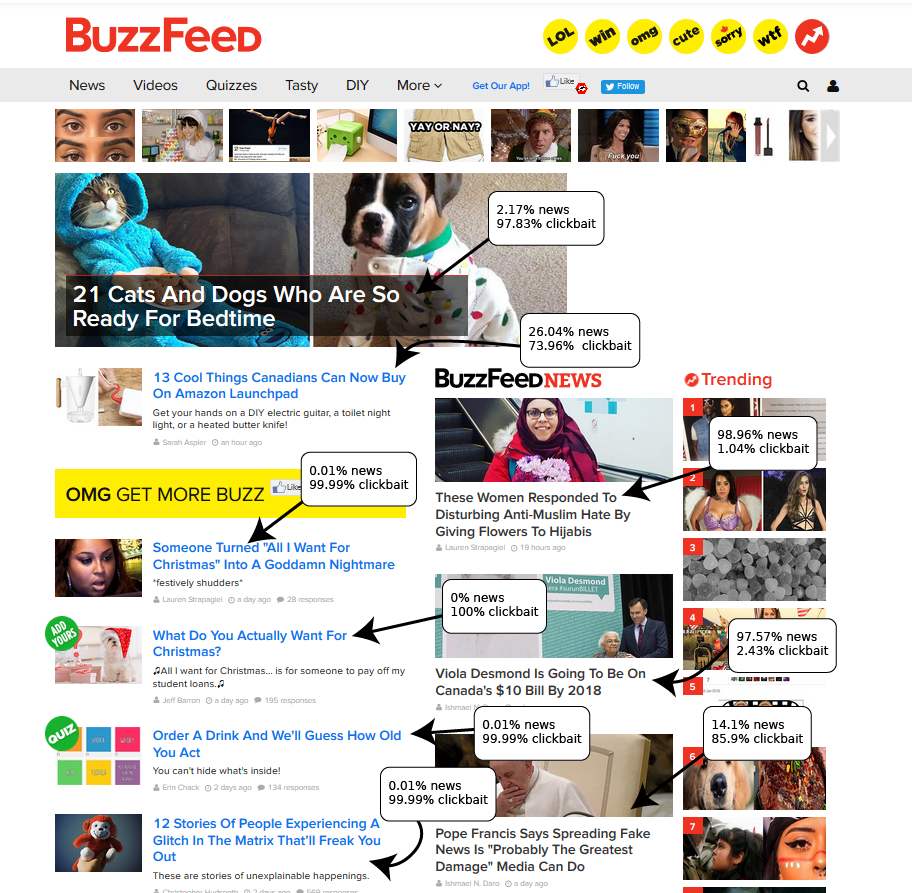
\includegraphics[width=12cm]{kapitel2/clickbait.png}
  \caption[Beispiel von Clickbait]{Beispiel von Clickbait}
  \label{Kap2:ClickBait}
\end{figure}


\begin{figure}[ht]
  \centering
  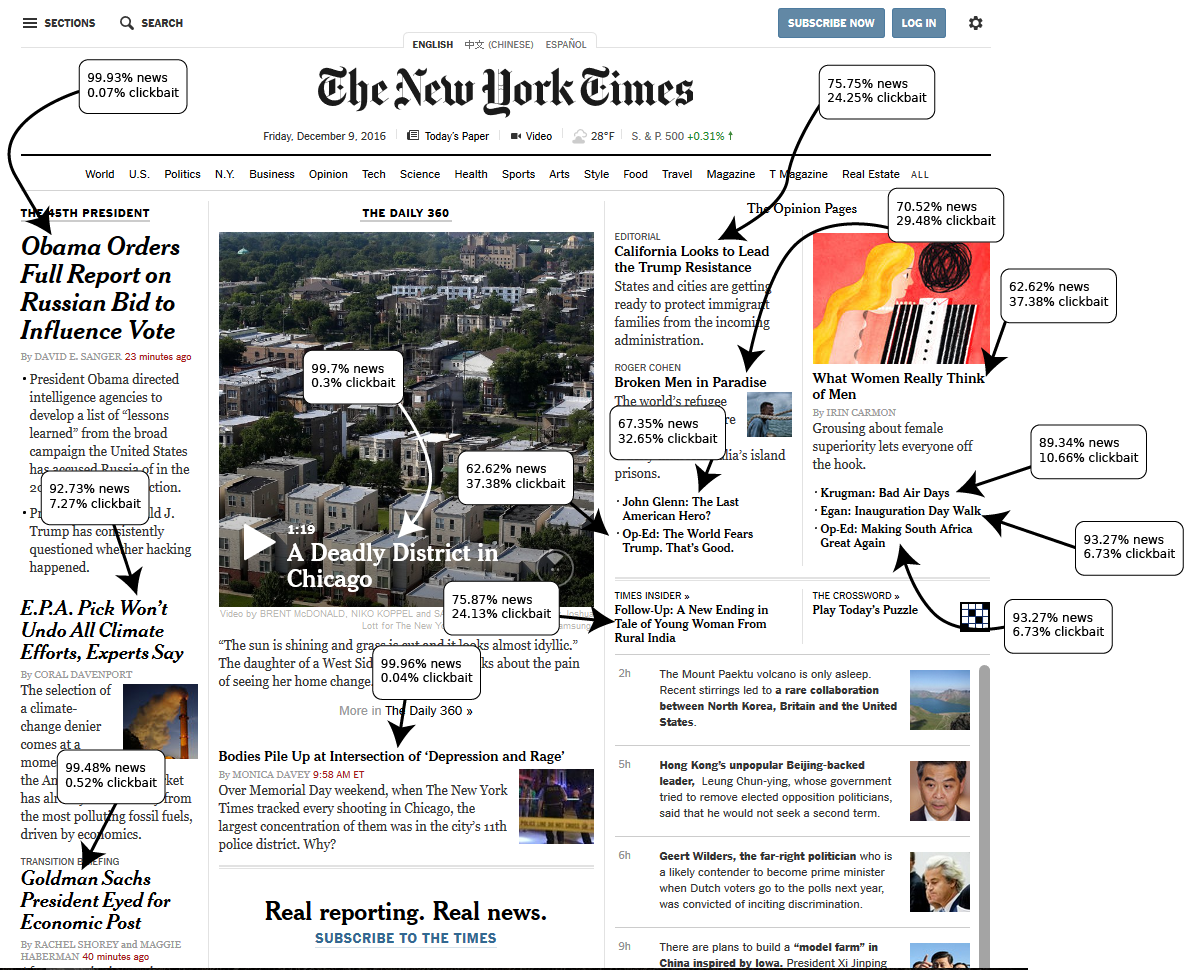
\includegraphics[width=12cm]{kapitel2/news.png}
  \caption[Beispiel von \enquote{normalen} Nachrichten]{Beispiel von \enquote{normalen} Nachrichten}
  \label{Kap2:News}
\end{figure}


\section{Lösungsansatz}
Textklassifizierung ist eine gängige Art, wie man \enquote{gute} von \enquote{bösen} Texten unterscheiden kann. Es ist allerdingt nicht praktisch ein großes Sprachmodell wie GPT-3 Browserkompatible zu machen. Erstens ist es völlig \enquote{overkill} für ein solches Problem ein Sprachmodell zu benutzen und zweitens passen diese großen Modelle nicht in den Browser, da die Ladezeit nicht praktisch ist.

Mit dieser Arbeit möchte ich ein Modell erstellen, um Clickbait Überschriften zu erkennen. Es wäre Hilfreich, wenn es ein Dienst gibt, welches eine Überschrift liest und dem Benutzer vorhersagt, ob es sich um Clickbait handelt oder nicht. So kann der Nutzer seine Zeit sparen und muss nicht auf die Seite gehen. Das Hauptprodukt ist dabei dieser Dienst, welches ganz einfach in jede HTML-Seite importiert werden kann. Dieser Dienst muss klein und schnell und gute dabei möglichst Ergebnisse liefern.

\section{Methodik}

Der erste theoretische Teil ist mathematisch/statistsch geprägt. Der zweite theoretische Teil beschäftigt sich mit der Sprache. Es wird nicht scharf zwischen den beiden Kapiteln getrennt, da diese viele Überlappungen haben werden. Ich werde ein Modell in TensorFlow.js entwickeln. Dieses Modell soll möglichst klein sein und schnell sein. Um mit TensorFlow.js arbeiten zu können muss der Text in Vektoren umgewandelt werden. Es gibt bereits ein Datensatz \footnote{https://www.kaggle.com/atechnohazard/clickbait-classifier-using-lstm} welches dafür verwendet werden kann. Clickbaits haben ein Muster, das Modell soll dieses Muster erkennen und mit einer relativ hohen Wahrscheinlichkeit sagen, ob es Clickbait ist. Mit einem Versuchsaufbau soll das Modell getestet und analysiert werden. Schließlich soll das Modell in die Browser-Umgebung gebracht und mittels eines minimalistischen React Frontends angeboten werden.

\begin{figure}[ht]
  \centering
  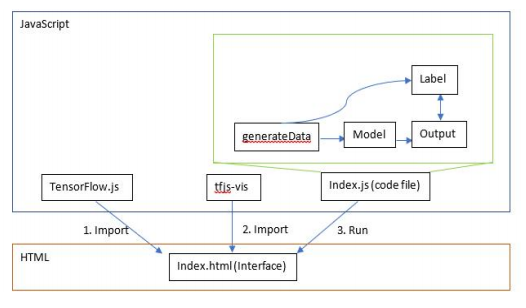
\includegraphics[width=12cm]{kapitel2/beispiel.png}
  \caption[Beispiel einer Systemarchitektur]{Beispiel einer Systemarchitektur entnommen aus \cite{cho2019shop}. Der Client bekommt beim laden der Seite, neben dem HTML, CSS und dem JavaScript, welches für das Frontend nötig ist, ein weiteres Script, welches die TensorFlow.js API bereitstellt. Die Berechnung findet im Browser, beim Client statt, wo auch das Modell sich befindet.}
  \label{Kap2:SystemArchitektur}
\end{figure}
 
\section{Wissenschaftlicher Beitrag}
\begin{itemize}
  \item Den Stand der Technik in Bezug auf Deep Learning und Worteinbettungen zeigen
  \item Implementierung eines NLP-Problemes im Browser ohne zusätzliche Software oder Plugins, mit TensorFlow.js
  \item Optimierung des Browsers für Deep Learning 
  \item Auswahl des optimalen Modells und der Trainingsmethode
  \item Produktion eines Dienstes, um Clickbait Nachrichten vorzubeugen
\end{itemize}

\section{Einstiegsliteratur}

\begin{itemize}
  \item \cite{Kaur2020a}
  \item \cite{Chavan2019}
  \item \cite{vorakitphan2018clickbait}
  \item \cite{Anand2017}
  \item \cite{gairola2017neural}
  \item \cite{kumar2018identifying}
  \item \cite{glenski2017fishing}
  \item \cite{chawda2019novel}
  \item \cite{seopredicting}
  \item \cite{cho2019shop}
  \item \cite{roberts2018magenta}
  \item \cite{aggarwal2012survey}
  \item \cite{kowsari2019text}
  \item \cite{korde2012text}
  \item \cite{altinel2018semantic}
  \item \cite{nordberg2020crucial}
  \item \cite{raamkumar2020use}
  \item \cite{rivera2020identifying}
  \item \cite{nguyen2020real}
  \item \cite{zhang2015character}
  \item \cite{kiranyaz20191d}
  \item \cite{severyn2015unitn}
  \item \cite{severyn2015twitter}
  \item \cite{zhao2019speech}
  \item \cite{eren2019generic}
\end{itemize}

\section{Grobgliederung}
\renewcommand{\labelenumii}{\theenumii}
\renewcommand{\theenumii}{\theenumi.\arabic{enumii}.}

\begin{enumerate}

  \item Einleitung
  \begin{enumerate}
    \item Motivation
    \item Wissenschaftlicher Beitrag
    \item Struktur der Arbeit
  \end{enumerate}

  \item Neuronale Netze
  \begin{enumerate}
    \item Einleitung
    \item Arten des Neuronalen Lernens
    \item Netzwerkparameter und Hyperparameter
    \item Aktivierungsfunktionen
    \item Verlustfunktion
    \item Optimizer
    \item Epochen
    \item TensorFlow.js
    \item Schluss
  \end{enumerate}

  \item Die natürliche Sprache
  \begin{enumerate}
    \item Einleitung
    \item Vektorisierung des Textes durch Encoding
    \item Worteinbettungen
    \item 1d CNN
    \item Schluss
  \end{enumerate}

  \item Aktueller Forschungsstand
  \begin{enumerate}
  \item Einleitung
  \item Clickbaits und Deep Learning Ansätze
  \item TensorFlow.js 
  \item Worteinbettungen
  \end{enumerate}

  \item Methodik
  \begin{enumerate}
    \item Einleitung
    \item Die Systemarchitektur
    \item JavaScript
    \item Explorative Datenanalyse
    \item Datenverarbeitung und Feature Engineering
    \item Modelling
    \item Das Zusammenbringen des Modells mit dem Frontend
    \item Schluss
  \end{enumerate}

  \item Versuchsaufbau und Diskussion der Ergebnisse
  \begin{enumerate}
    \item Einleitung
    \item Anpassung der Netzwerkparameter und Hyperparameter
    \item Leistungsmessungen
    \item Vergleich und Darstellung der Ergebnisse
    \item Schluss
  \end{enumerate}

  \item Schluss
  \begin{enumerate}
    \item Fazit zum Forschungsbeitrag
    \item Abschließende Gedanken
    \item Zukunft der Arbeit
  \end{enumerate}
\end{enumerate}




% \section{Hervorhebungen}
% \label{Einleitung:Textauszeichnungen}

% Achten Sie bitte auf die grundlegenden Regeln der Typographie\index{Typographie}\footnote{Ein Ratgeber in allen Detailfragen ist \cite{Forssman2002}.}, wenn Sie Ihren Text schreiben. Hierzu gehören z.\,B. die Verwendung der richtigen "`Anführungszeichen"' und der Unterschied zwischen Binde- (-), Gedankenstrich (--) und langem Strich (---). Sie erhalten den Bindestrich in \LaTeX{} mit \verb+-+, den Gedankenstrich mit \verb+--+ und den langen Strich mit \verb+---+.

% Wenn Sie Text hervorheben wollen, dann setzten Sie ihn mit \verb+\textit+ \textit{kursiv} (Italic) und nicht \textbf{fett} (Bold). Fettdruck ist Überschriften vorbehalten; im Fließtext stört er den Lesefluss. Das \underline{Unterstreichen} von Fließtext ist im gesamten Dokument tabu und kann maximal bei Pseudo"=Code vorkommen.\index{Hervorhebungen}


% \section{Anführungszeichen}

% Deutsche Anführungszeichen werden mit \verb+"`+ und \verb+"'+ erzeugt: "`dieser Text steht in \glq Anführungszeichen\grq; alles klar?"'. Englische Anführungszeichen hingegen mit \verb+``+ und \verb+''+: ``this is an `English' quotation''. Beachten Sie, dass Sie in Zitaten immer die zur Sprache passenden Anführungszeichen verwenden. Die Verwendung von \verb+"+ ist für Anführungszeichen immer falsch und führt bei \LaTeX{} zu seltsamen "Effekten".

% Um sich diesen Ärger zu sparen, biete sich die Verwendung des Paketes \textit{csquotes} und des Kommandos \verb+\enquote+ an. Hierdurch werden die Anführungszeichen korrekt für die eingestellte Sprache gesetzt und Sie müssen sich \enquote{keine Sorgen mehr über die \enquote{Anführungszeichen} machen}.


% \section{Abkürzungen}
% \index{Abkürzungen}
% \index{Abbreviation|see{Abkürzungen}}

% Eine \ac{ABK} (\verb+\ac{ABK}+) wird bei der ersten Verwendung ausgeschrieben. Danach nicht mehr: \ac{ABK}. Man kann allerdings mit \verb+\acl+ die Langform explizit anfordern (\acl{ABK}) oder mit \verb+\acs+ die Kurzform (\acs{ABK}) oder mit \verb+\acf+ auch noch einmal die Definition (\acf{ABK}).

% Beachten Sie, dass bei Abkürzungen, die für zwei Wörter stehen, ein kleines Leerzeichen nach dem Punkt kommt: z.\,B. bzw. \zb{} und d.\,h. bzw. \dahe{}. Das Template bietet hierfür die beiden Makros \verb+\zb{}+ und \verb+\dahe{}+.


% \section{Querverweise}

% Querverweise auf eine Kapitelnummer macht man im Text mit \verb+\ref+ (Kapitel~\ref{Einleitung:Textauszeichnungen}) und auf eine bestimmte Seite mit \verb+\pageref+ (Seite~\pageref{Einleitung:Textauszeichnungen}). Man kann auch den Befehl \verb+\autoref+ benutzen, der automatisch die Art des referenzierten Elements bestimmt (\zb{} \autoref{Einleitung:Textauszeichnungen} oder \autoref{Kap2:Kopplungsformen}).


% \section{Fußnoten}

% Fußnoten werden einfach mit in den Text geschrieben und zwar genau an die Stelle\footnote{An der die Fußnote auftauchen soll}. Hierzu dient der Befehl \verb+\footnote{Text}+.


% \section{Tabellen}

% Tabellen werden normalerweise ohne vertikale Striche gesetzt, sondern die Spalten werden durch einen entsprechenden Abstand voneinander getrennt.\footnote{Siehe \cite[S. 89]{Willberg1999}.} Zum Einsatz kommen ausschließlich horizontale Linien (siehe Tabelle~\ref{Kap2:Kopplungsformen}).

% \begin{table}[h]
%   \caption{Ebenen der Kopplung und Beispiele für enge und lose Kopplung}
%   \label{Kap2:Kopplungsformen}
%   \renewcommand{\arraystretch}{1.2}
%   \centering
%   \sffamily
%   \begin{footnotesize}
%     \begin{tabular}{l l l}
%     \toprule
%     \textbf{Form der Kopplung} & \textbf{enge Kopplung} & \textbf{lose Kopplung}\\
%     \midrule
%     Physikalische Verbindung	&	Punkt-zu-Punkt	& 	über Vermittler\\
%     Kommunikationsstil	&	synchron		&	asynchron\\
%     Datenmodell	&	komplexe gemeinsame Typen	&	nur einfache gemeinsame Typen\\
%     Bindung	&	statisch		&	dynamisch\\
%     \bottomrule
%     \end{tabular}
%   \end{footnotesize}
%   \rmfamily
% \end{table}

% Eine Tabelle fließt genauso, wie auch Bilder durch den Text. Siehe Tabelle~\ref{Kap2:Kopplungsformen}.

% Manchmal möchte man Tabellen, in denen der Text in der Tabellenspalte umbricht. Hierzu dient die Umgebung \texttt{tabularx}, wobei \texttt{L} eine Spalte mit Flattersatz und \texttt{X} eine mit Blocksatz definiert. Die Breite der Tabelle kann über den Faktor vor \verb+\textwidth+ angegeben werden.

% \begin{table}[h]
%   \caption{Teildisziplinen der Informatik}
%   \label{Kap2:Teildisziplinen}
%   \renewcommand{\arraystretch}{1.2}
%   \centering
%   \sffamily
%   \begin{footnotesize}
%     \begin{tabularx}{0.9\textwidth}{l X L}
%       \toprule
%       \textbf{Gebiet} & \textbf{Definition} & \textbf{Beispiel}\\
%       \midrule
%       \emph{Praktische Informatik} & Informatik-Disziplinen, welche sich vorwiegend mit der Entwicklung und Anwendung der Software-Komponenten befassen & Programmentwicklung, Compilerbau; im Aufbau von z.B. Informationssystemen und Netzwerken ergeben sich Überlappungen mit der technischen Informatik \\
%       \emph{Technische Informatik} & Informatik-Disziplinen, welche sich vorwiegend mit der Entwicklung und Anwendung der Hardware-Komponenten befassen & Digitaltechnik, Mikroprozessortechnik \\
%       \emph{Theoretische Informatik} & Informatik-Disziplinen, welche sich mit der Entwicklung von Theorien und Modellen der Informatik befassen und dabei viel Substanz aus der Mathematik konsumieren & Relationenmodell, Objekt-Paradigmen, Komplexitätstheorie, Kalküle \\
%       \emph{Angewandte Informatik} & Informatik als instrumentale Wissenschaft & Rechtsinformatik, Wirtschaftsinformatik, Geoinformatik \\
%       \bottomrule
%     \end{tabularx}
%   \end{footnotesize}
%   \rmfamily
% \end{table}


% \section{Harveyballs}

% \begin{quote}
%     Harvey Balls sind kreisförmige Ideogramme, die dazu dienen, qualitative Daten anschaulich zu machen. Sie werden in Vergleichstabellen verwendet, um anzuzeigen, inwieweit ein Untersuchungsobjekt sich mit definierten Vergleichskriterien deckt. \parencite{Wikipedia_HarveyBalls}
% \end{quote}

% \begin{table}[h]
%   \caption{Beispiel für Harvey Balls}
%   \label{tab:harveyexample}
%   \centering
%   \begin{tabular}{lccc}
%     \toprule
%     & Ansatz 1 & Ansatz 2 & Ansatz 3\\
%     \midrule
%     Eigenschaft 1	& \harveyBallNone & \harveyBallQuarter & \harveyBallHalf \\
%     Eigenschaft 2	& \harveyBallHalf & \harveyBallThreeQuarter & \harveyBallFull \\
%     Eigenschaft 3	& \harveyBallFull & \harveyBallThreeQuarter & \harveyBallQuarter\\
%     \bottomrule
%   \end{tabular}
% \end{table}


% \section{Aufzählungen}

% Aufzählungen sind toll.

% \begin{itemize}
%   \item Ein wichtiger Punkt
%   \item Noch ein wichtiger Punkt
%   \item Ein Punkt mit Unterpunkten
%     \begin{itemize}
%       \item Unterpunkt 1
%       \item Unterpunkt 2
%     \end{itemize}
%   \item Ein abschließender Punkt ohne Unterpunkte
% \end{itemize}


% Aufzählungen mit laufenden Nummern sind auch toll.

% \begin{enumerate}
%   \item Ein wichtiger Punkt
%   \item Noch ein wichtiger Punkt
%   \item Ein Punkt mit Unterpunkten
%     \begin{enumerate}
%       \item Unterpunkt 1
%       \item Unterpunkt 2
%     \end{enumerate}
%   \item Ein abschließender Punkt ohne Unterpunkte
% \end{enumerate}
 % Externe Datei einbinden
\chapter{Einbinden von Grafiken, Sourcecode und Anforderungen}
\label{Kap3}

\section{Bilder}

Natürlich können auch Grafiken und Bilder eingebunden werden, siehe z.\,B. Abbildung~\ref{Kap2:NasaRover}.

\begin{figure}[ht]
  \centering
  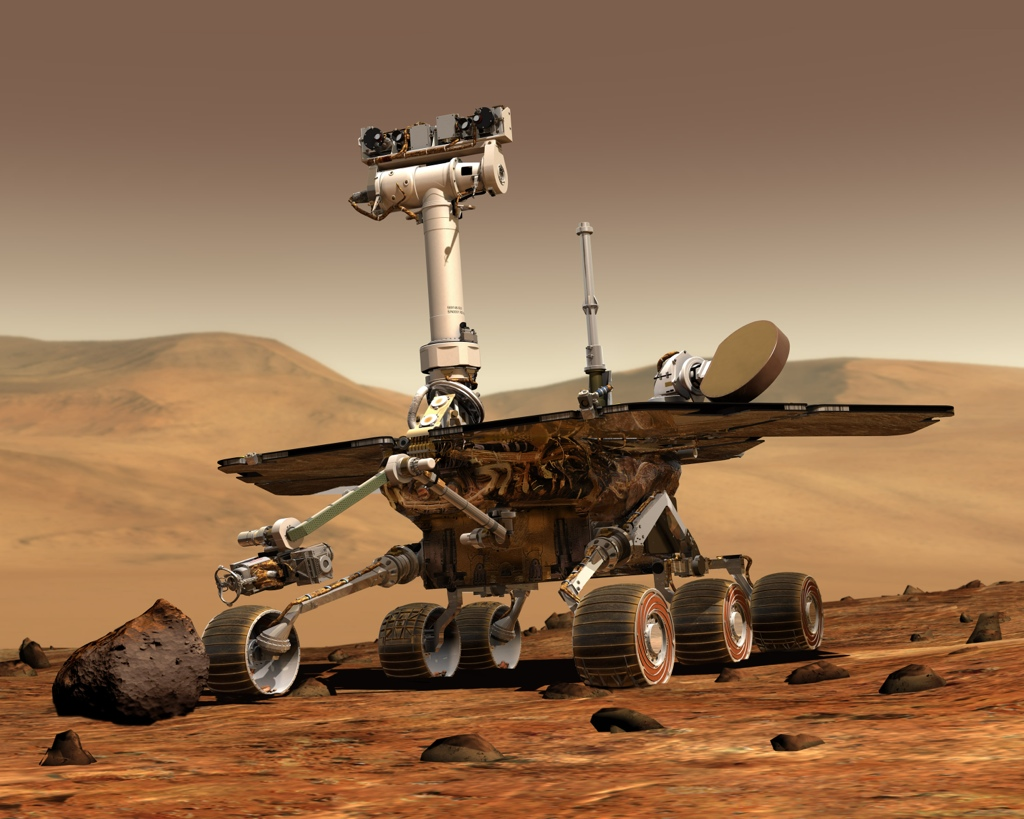
\includegraphics[width=6cm]{kapitel3/nasa_rover}
  \caption{Ein Nasa Rover}
  \label{Kap2:NasaRover}
\end{figure}

Man kann sich auch selbst ein Makro für das Einfügen von Bildern schreiben:

\bild{kapitel3/modell_point_to_point}{6cm}{Point to Point}

\begin{sidewaysfigure}
 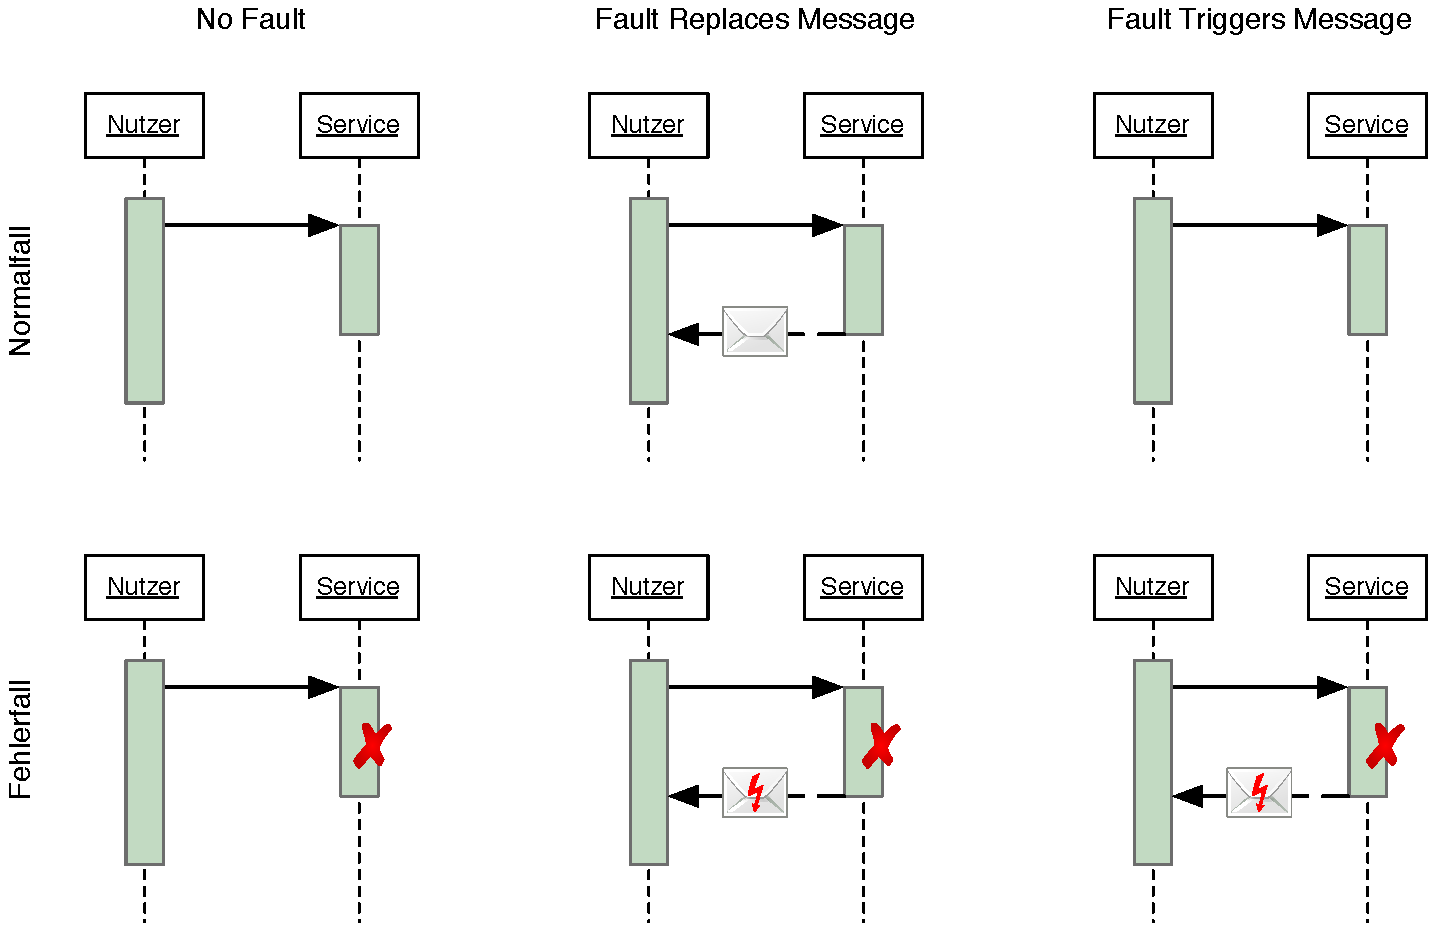
\includegraphics[width=22cm]{kapitel3/ws-wsdl20-fehler}
  \caption{Sehr große Grafiken kann man drehen, damit sie auf die Seite passen}
  \label{Kap2:wsdl-fehler}
\end{sidewaysfigure}

\clearpage % Alle Bilder, die bisher kamen ausgeben


\section{Formelsatz}

Eine Formel gefällig? Mitten im Text $a_2 = \sqrt{x^3}$ oder als eigener Absatz (siehe Formel~\ref{Formel}):

\begin{equation}
\begin{bmatrix}
   1 &  4 &  2 \\
   4 &  0 & -3
\end{bmatrix}
        \cdot
\begin{bmatrix}
   1 &  1 &  0 \\
  -2 &  3 &  5 \\
   0 &  1 &  4
\end{bmatrix}
       {=}
\begin{bmatrix}
  -7 &  15 &  28 \\
   4 &   1 & -12
\end{bmatrix}
\label{Formel}
\end{equation}


\section{Sourcecode}

Man kann mit Latex auch ganz toll Sourcecode in den Text aufnehmen.

\subsection{Aus einer Datei}

\lstinputlisting[firstline=2,language=Java,caption={Crypter-Interface},label=lst:CrypterInterface]{\srcloc/Crypter.java}


\subsection{Inline}

\begin{lstlisting}[language=Java,caption=Methode checkKey()]
    /**
     * Testet den Schlüssel auf Korrektheit: Er muss mindestens die Länge 1
     * haben und darf nur Zeichen von A-Z enthalten.
     *
     * @param key zu testender Schlüssel
     * @throws CrypterException wenn der Schlüssel nicht OK ist.
     */
    protected void checkKey(Key key) throws CrypterException {

        // Passt die Länge?
        if (key.getKey().length == 0) {
            throw new CrypterException("Der Schlüssel muss mindestens " +
                    "ein Zeichen lang sein");
        }

        checkCharacters(key.getKey(), ALPHABET);
    }
\end{lstlisting}


\section{Anforderungen}

Anforderungen im Format des Volere"=Templates (Snowcards) \autocite{Volere} können per Makro eingefügt werden. Das Label wird automatisch mit der Nummer erstellt, d.\,h. Sie können auf die Tabelle mit dieser referenzieren (siehe \autoref{F52}).

\snowcard % Snowcard einbinden (Anpassungen in titelblatt.tex)
   {F52} % Nummer des Requirements
   {F} % Art
   {Hoch} % Priorität
   {User Authentifizierung} % Titel
   {Interview mit Abteilungsleiter} % Herkunft (Optional)
   {F12} % Konflikte (Optional)
   {Der Benutzer ist in der Lage sich über seinen
    Benutzernamen und sein Passwort am System anzumelden} % Beschreibung
   {Ein Benutzer kann sich mit seinem firmenweiten Benutzernamen und
   Passwort über die Anmeldemaske anmelden und hat Zugriff auf die
   Funktionen des Systems} % Fit-Kriterium (Optional)
   {Benutzerhandbuch des Altsystems} % Material (Optional)

Ebenso können Sie nicht"=funktionale Anforderungen mit Hilfe von Quality Attribute Scenarios (vgl. \autoref{NF11}) darstellen. Zu Details siehe \autocite{Barbacci2003}.

\qas % Quality-Attribute Scenario einbinden (Anpassungen in titelblatt.tex)
   {NF11} % Nummer des Requirements
   {Hoch} % Priotität
   {Performance des Jahresabschlusses} % Titel
   {Endbenutzer} % Quelle
   {Startet einen Jahresabschluss} % Stimulus
   {Buchhaltungssystem} % Artefakt
   {Das System befindet sich im normalen Betriebszustand} % Umgebung
   {Jahresabschluss ist durchgeführt und kann als PDF abgerufen werden} % Antwort
   {10 Minuten} % Antwort-Maß

Die Abgrenzung von funktionalen und nicht-funktionalen Anforderungen ist nicht immer einfach und bereitet manchen Studierenden Probleme. Als Hilfestellung kann die von der ISO25010 \autocite{ISO25010} zur Verfügung gestellte Liste dienen, siehe \autoref{kapitel3/iso25010}.

\bild{kapitel3/iso25010}{14cm}{Qualitätsmodell für Software-Produkte nach ISO25010}

\citeauthor{Bass2003} listen in \autocite{Bass2003} eine ähnliche Liste von Kategorien für nicht-funktionalen Anforderungen auf, die ebenfalls als Richtschnur dienen kann. Diese sind:

\begin{itemize}
  \item \textit{Verfügbarkeit} \textit{(availability)} -- umfasst Zuverlässigkeit (reliability), Robustheit (robustness), Fehlertoleranz (fault tolerance) und Skalierbarkeit (scalability)
  \item \textit{Anpassbarkeit} \textit{(modifiability)}, umfasst Wartbarkeit (maintainability), Verständlichkeit (understandability) und Portabilität (portability).
  \item \textit{Performanz} \textit{(performance)}
  \item \textit{Sicherheit} \textit{(security)}
  \item \textit{Testbarkeit} \textit{(testability)}
  \item \textit{Bedienbarkeit} \textit{(usability)}
\end{itemize}
 % Externe Datei einbinden
\chapter{Checkliste}
\label{Kap4}

Die folgende Checkliste kann dazu dienen, die Arbeit auf die wichtigsten Bewertungskriterien zu prüfen. Jeder Dozent hat andere Kriterien, die unten aufgeführten dürften aber für die meisten Dozenten gültig sein.

\section{Form und Sprache}

\begin{checklist}
  \footnotesize
  \item \textbf{Aufbau}: Die Arbeit ist nach wissenschaftlichen Prinzipien aufgebaut (wesentliche Teile vorhanden, Nummerierung/Verweise korrekt, Verzeichnisse vorhanden).
    \begin{checklist}
        \item \textit{Wesentliche Teile}: Die folgenden Elemente der Arbeit sind vorhanden: Titelblatt, Abstract/Zusammenfassung, Einleitung, Hauptteil, Fazit/Ausblick.
        \item \textit{Nummerierung/Verweise}: Das Nummerierungsschema wird konsistent über die gesamte Arbeit durchgehalten, die Verweise auf die verschiedenen Elemente (Abbildungen, Tabellen etc.) sind korrekt.
        \item \textit{Verzeichnisse}: Die Arbeit enthält alle relevanten Verzeichnisse: Inhaltsverzeichnis, Literaturverzeichnis, Abbildungsverzeichnis, Tabellenverzeichnis, eventuell Glossar.
    \end{checklist}
  \item \textbf{Sprache}: Die verwendete Sprache entspricht wissenschaftlichen Ansprüchen.
    \begin{checklist}
        \item \textit{Begriffe und Definitionen}: Begriffe werden einheitlich und konsistent verwendet. Neue Begriffe werden definiert und mit Literatur hinterlegt.
        \item \textit{Abkürzungen}: Alle Abkürzungen werden eingeführt und erläutert. Abkürzungen werden bei der ersten Verwendung ausgeschrieben und in einem Abkürzungsverzeichnis geführt. Es werden keine unüblichen oder selbst erfunden Abkürzungen verwendet. Ein Glossar kann verwendet werden, um Begriffe noch einmal kompakt darzustellen.
        \item \textit{Rechtschreibung}: Die Arbeit ist frei von Rechtschreibungs-, Zeichensetzungs- und Grammatikfehlern.
    \end{checklist}
  \item \textbf{Formatierung, Typographie}: Die Formatierung der Arbeit ist korrekt und aus typographischer Sicht einwandfrei. \textit{Wenn Sie dieses Template korrekt verwenden, sollte dieser Punkt automatisch durch die Verwendung von \LaTeX \ erledigt sein.}
    \begin{checklist}
        \item \textit{Korrekte Typographie}: Schriftarten werden korrekt verwendet (nicht mehr als 2 Fonts), der Zeilenabstand ist passend, die Ränder sind ausreichend, der Satz ist korrekt.
        \item \textit{Satz von Abbildungen, Tabellen etc.}: Abbildungen sind in der richtigen Auflösung dargestellt, die Tabellen sind korrekt gesetzt, mathematische Formeln und Symbole sind sauber dargestellt.
    \end{checklist}
  \item \textbf{Abbildungen}: Abbildungen werden in ausreichendem Umfang zur Förderung des Verständnisses eingesetzt. Sie werden korrekt im Text referenziert und sind, wo immer möglich, in einer Standardnotation erstellt.
    \begin{checklist}
        \item \textit{Ausreichende Verwendung}: Komplizierte Sachverhalte werden durch Abbildungen verdeutlicht. Es werden genug Abbildungen eingesetzt, um die wichtigsten Sachverhalte zu erklären.
        \item \textit{Verständnisförderung}: Abbildungen dienen nicht als Schmuck, sondern um komplizierte Sachverhalte zu verdeutlichen.
        \item \textit{Einbindung in den Text}: Der Text muss auch ohne Abbildungen verständlich sein, die Abbildungen helfen Sachverhalte aus dem Text besser darzustellen. Der Text referenziert die Abbildung korrekt.
        \item \textit{Standardnotation, Legende}: Die Abbildungen verwenden Standard"=Notationen wie UML, FMC etc. Wo keine Standardnotation eingesetzt wird, ist eine Legende vorhanden, um die Bildelemente zu erläutern.
    \end{checklist}
  \item \textbf{Zitate}: Quellen werden konsistent nach einer gängigen Zitierweise zitiert und sind vollständig im Literaturverzeichnis angegeben.
    \begin{checklist}
        \item \textit{Zitierweise}: Die Zitierweise in der gesamten Arbeit folgt einem einheitlichen Schema, z.B. IEEE, DIN, Chicago.
        \item \textit{Vollständigkeit}: Alle Zitate sind als solche kenntlich gemacht und die Quelle wird vollständig angegeben, und Plagiate werden vermieden.
    \end{checklist}
  \item \textbf{Schreibstil}: Lebendiger, wissenschaftlicher und verständlicher Schreibstil.
    \begin{checklist}
        \item \textit{Wissenschaftlichkeit}: Der Text ist im Präsenz geschrieben, es wird die dritte Person verwendet, Fachausdrücke werden korrekt verwendet, Fremdwörter und Amerikanismen werden richtig eingesetzt.
        \item \textit{Verständlichkeit}: Abschweifungen und Wiederholungen werden vermieden, statt dessen werden präzise und übersichtliche Sätze verwendet.
        \item \textit{Lebendigkeit}: Der Text der Arbeit zeichnet sich durch eine gute Wortwahl, Sprachbilder, einen angemessenen Satzbau und eine hohe Variabilität aus.
    \end{checklist}
\end{checklist}

\section{Inhalt}

\begin{checklist}
  \footnotesize
  \item \textbf{Gliederung}: Die Gliederung ist vollständig, konsistent und sachlogisch mit angemessener Struktur und Tiefe.
    \begin{checklist}
        \item \textit{Konsistenz und Vollständigkeit}: Auf einer Ebene stehen keine Punkte alleine, die Gliederungspunkte orientieren sich an der Argumentationskette.
        \item \textit{Angemessene Tiefe}: Die Größe der einzelnen Unterpunkte ist vom Umfang her ähnlich. Es gibt keine Gliederungspunkte, die nur aus ein bis zwei Sätzen bestehen.
    \end{checklist}
  \item \textbf{Grundlagen}: Es werden alle relevanten Grundlagen gelegt. Der State"=of"=the"=art und der State"=of"=practice werden dargelegt.
    \begin{checklist}
        \item \textit{Umfang}: 1/3 des Hauptteils ist ein gutes Maß für eine ausreichende Darstellung der Grundlagen.
        \item \textit{Begriffe und Methoden}: Begriffe und Methoden sind definiert, und Literatur zu den Definitionen ist angegeben.
        \item \textit{State-of-the-art}: Der Stand des verfügbaren Wissens wird dargestellt, analysiert und kritisch beurteilt (state-of-the-art). Bei theoretischen Arbeiten kann ein eigenes Kapitel \enquote{verwandte Arbeiten} nötig sein, um den state"=of"=the"=art darzustellen.
        \item \textit{State-of-practice}: Bei praktischen Arbeiten, die in der Industrie geschrieben werden, kann es nötig sein, auch das Vorgehen im Unternehmen zu erläutern.
    \end{checklist}
  \item \textbf{Methodik/Lösung}: Die gewählte Methodik bzw. Lösung ist für das Problem adäquat.
    \begin{checklist}
        \item \textit{Anforderungen an die Lösung}: Die von der Lösung zu erfüllenden Anforderungen werden dargestellt. Wo nötig wird dies auf Grundlage eines sauberen Requirements"=Engineerings durchgeführt.
        \item \textit{Erläuterung des Lösungsansatzes}: Der gewählte Lösungsansatz wird ausführlich erläutert und verständlich dargestellt.
        \item \textit{Eignung zur Lösung der Aufgabe}: Die gewählte Lösung ist geeignet, um das beschriebene Problem zu lösen.
        \item \textit{Hypothesen}: Es sind ggf. Hypothesen gebildet worden; diese sind erläutert, und es sind Kriterien identifiziert worden, mit deren Hilfe man die Hypothesen falsifizieren kann.
        \item \textit{Alternativen}: Es werden Alternativen zur vorgeschlagenen Lösung diskutiert. Die eigene Lösung wird nicht als einzige mögliche dargestellt, sondern es werden auch andere mögliche Lösungen vorgestellt und bewertet.
        \item \textit{Begründung}: Alternativen und Kriterien für die Auswahl dieser Lösung werden dargestellt.
        \item \textit{Vorteile der Lösung}: Es wird dargestellt, wieso die entwickelt Lösung vorteilhafter ist als die bisherigen Ansätze. Diese Darstellung erfolgt auf Basis des Lösungsansatzes. Eine konkrete Validierung der Implementierung erfolgt ggf. in späteren Kapiteln.
    \end{checklist}
  \item \textbf{Logik der Argumentationskette}: Die Argumentation ist logisch und nachvollziehbar. Sie ist frei von logischen Fehlschlüssen.
  \item \textbf{Implementierung}: Wenn eine Implementierung der Lösung erfolgt, so wird die Implementierung beschrieben. Die Darstellung der Implementierung kann knapp ausfallen. Wichtig ist der Lösungsansatz, nicht die konkrete Umsetzung.
  \item \textbf{Validierung}: Die vorgeschlagene Lösung wird ggf. empirisch verprobt.
    \begin{checklist}
        \item \textit{Vorgehensweise}: Die Vorgehensweise zur Validierung der Lösung / Hypothesen ist beschrieben und geeignet, relevante Aspekte der Lösung zu überprüfen.
        \item \textit{Empirische Analyse}: Die Erfassungsmethode wird dargestellt und die Daten werden nach den Grundsätzen ordnungsgemäßer Laborpraxis gesammelt und statistisch korrekt ausgewertet.
        \item \textit{Verprobung}: Die Lösung wird an einem praktischen Beispiel verprobt, und es werden wissenschaftlich korrekte Schlüsse aus der Anwendung gezogen.
        \item \textit{Zielerreichung}: Funktioniert die gewählte Lösung nach der Implementierung? Wie weit wurde das Ziel erreicht? Falls nicht, gibt es nachvollziehbare Gründe dafür und wurden diese dargestellt?
    \end{checklist}
  \item \textbf{Diskussion}: Die Lösung und ihre Validierung wird kritisch und im Kontext möglicher Alternativen diskutiert und bewertet.
    \begin{checklist}
        \item \textit{Kritische Reflektion}: Grenzen und Schwächen der eigenen Ergebnisse werden beleuchtet.
        \item \textit{Ableitung von Konsequenzen}: Die Konsequenzen aus den Ergebnissen für die Wissenschaft und Praxis sind beschrieben.
    \end{checklist}
  \item \textbf{Quellenarbeit}: Es werden hochwertige Quellen in ausreichendem Umfang genutzt und kritisch hinterfragt. Eventuell vorhandene Quellen aus dem Unternehmen werden ebenfalls berücksichtigt.
    \begin{checklist}
        \item \textit{Umfang}: Der Umfang an Quellen richtet sich stark nach Thema und Art der Arbeit. Bei einer Bachelorarbeit sind mindestens 20 Primärquellen und entsprechend viele Sekundärquellen üblich, bei einer Masterarbeit deutlich mehr.
        \item \textit{Wissenschaftliche Qualität}: Nicht zitierfähig sind Internet"=Quellen, Wikipedia"=Einträge sowie andere Bachelor- oder Masterarbeiten (sofern nicht veröffentlicht). Das ausschließliche Zitieren von Lehrbüchern ist problematisch. Aktuelle wissenschaftliche Artikel und Werke sollten in den Quellen auftauchen.
        \item \textit{Quellen \enquote{aus der Praxis}}: Wenn es im Unternehmen spezielle Quellen und Informationen gibt, so werden diese berücksichtigt, z. B. firmen- oder branchenspezifischer Informationen.
        \item \textit{Kritische Würdigung}: Quellen und Zitate werden kritisch hinterfragt und nicht einfach unreflektiert übernommen. Es gibt eine kritische Distanz bei der Quellenauswahl und Quellenauswertung.
    \end{checklist}
  \item \textbf{Fazit}: Es wird eine Zusammenfassung der Arbeit sowie Ausblick auf weitere mögliche Arbeiten im Themenfeld gegeben, etwa die Lösung ausstehender Probleme oder die Erfüllung zusätzlicher Anforderungen.
  \item \textbf{Umfang der Arbeit}: Richtgrößen: Bachelorarbeiten: 50--80 Seiten, Masterarbeiten: 60--100 Seiten, jeweils ohne Verzeichnisse und Anhang.
\end{checklist}

\section{Vor der Abgabe}

\begin{checklist}
  \footnotesize
  \item \textit{Korrektur}: Haben Sie einen Dritten die Arbeit lesen lassen und alle gefundenen Rechtschreib- und Zeichensetzungsfehler behoben?
  \item \textit{Literaturverzeichnis}: Sind im Literaturverzeichnis irrelevante Informationen entfernt? Beispielsweise bei Büchern unnötige Informationen über die Herkunft bei Google-Books oder bei Papern doppelte Angaben der DOI?
  \item \textit{Doppel- oder einseitiger Druck}: Entspricht die Einstellung des Templates dem Druck, d.\,h. ist das Template für doppelseitigen Druck eingestellt, wenn doppelseitig gedruckt werden soll und umgekehrt?
  \item \textit{Umschläge}: Sind die Umschläge vorhanden, um die Arbeit später zu binden? Die Umschläge können in der Hausdruckerei der Hochschule erworben werden.
  \item \textit{Copyshop}: Wissen Sie, wo Sie die Arbeit drucken werden? Die Hausdruckerei kann Ihre Arbeit nicht drucken.
  \item \textit{Exemplare}: Haben Sie geklärt, ob der Zweitkorrektor auch ein gedrucktes Exemplar möchte?
\end{checklist}
 % Externe Datei einbinden
% ------------------------------------------------------------------

\label{lastpage}

% Neue Seite
\cleardoublepage

% Backmatter mit normalem Zeilenabstand setzen
\singlespacing

% Römische Ziffern für die "Back-Matter", fortlaufend mit "Front-Matter"
\pagenumbering{roman}
\setcounter{page}{\value{frontmatterpage}}

% Abkürzungsverzeichnis
\addchap{\hsmaabbreviations}
% % Die längste Abkürzung kann in die eckigen Klammern
% % bei \begin{acronym} geschrieben, um einen hässlichen
% % Umbruch zu verhindern
% %
% % ACHTUNG: Sie müssen die Abkürzungen von Hand alphabetisch
% %          sortieren. Das passiert nicht automatisch.
% \begin{acronym}[IEEE]
% \acro{ABK}{Abkürzung}
% \acro{ACM}{Association of Computing Machinery}
% \acro{PDF}{Portable Document Format}
% \acro{IEEE}{Institute of Electrical and Electronics Engineers}
% \acro{ISO}{International Organization for Standardization}
% \end{acronym}


% Tabellenverzeichnis erzeugen
\cleardoublepage
\phantomsection
\addcontentsline{toc}{chapter}{\hsmalistoftables}
\listoftables

% Abbildungsverzeichnis erzeugen
\cleardoublepage
\phantomsection
\addcontentsline{toc}{chapter}{\hsmalistoffigures}
\listoffigures

% Listingverzeichnis erzeugen. Wenn Sie keine Listings haben,
% entfernen Sie einfach diesen Teil.
\cleardoublepage
\phantomsection
\addcontentsline{toc}{chapter}{\hsmalistings}
\lstlistoflistings

% Literaturverzeichnis erzeugen
\begingroup
\cleardoublepage
\begin{flushleft}
\let\clearpage\relax % Fix für leere Seiten (issue #25)
\printbibliography
\end{flushleft}
\endgroup

% Index ausgeben. Wenn Sie keinen Index haben, entfernen Sie einfach
% diesen Teil. Die meisten Abschlussarbeiten haben *keinen* Index.
\cleardoublepage
\phantomsection
\addcontentsline{toc}{chapter}{\hsmaindex}
\printindex

% Anhang. Wenn Sie keinen Anhang haben, entfernen Sie einfach
% diesen Teil.
\appendix
% \chapter{Erster Anhang}

% Hier ein Beispiel für einen Anhang. Der Anhang kann genauso in Kapitel und Unterkapitel unterteilt werden, wie die anderen Teile der Arbeit auch.

% \chapter{Zweiter Anhang}

% Hier noch ein Beispiel für einen Anhang.


\end{document}
